\documentclass[11pt]{article}

\usepackage[T1]{fontenc}
\usepackage{lmodern}
\usepackage[final]{microtype}
\usepackage[a4paper,margin=2.5cm]{geometry}
\usepackage{amsmath,amssymb}
\usepackage{graphicx}
\usepackage{booktabs}
\usepackage{tabularx}
\usepackage{enumitem}
\usepackage{xcolor}
\usepackage[font=small,labelfont=bf,labelsep=period]{caption}
\usepackage{float}
\usepackage[section]{placeins}
\usepackage{longtable}
\usepackage{listings}
\usepackage[numbers,sort&compress]{natbib}
\usepackage[colorlinks=true,linkcolor={blue!50!black},citecolor={blue!50!black},
  urlcolor={blue!60!black},pdftitle={Modelly: Fast and Reproducible Agent-Based Modelling in Python, with Calibration and Sensitivity Analysis Built In},
  pdfauthor={R\'emi Pelloux},pdfkeywords={agent-based modelling, Python, reproducibility, approximate Bayesian
  computation, global sensitivity analysis, distributed simulation, GPU, data assimilation,
  benchmarking, scientific software}]{hyperref}
\usepackage[capitalise,noabbrev]{cleveref}
\urlstyle{same}

\lstset{
  language=Python,
  basicstyle=\ttfamily\footnotesize,
  keywordstyle=\color[HTML]{0072B2},
  commentstyle=\color[HTML]{6B6B6B},
  stringstyle=\color[HTML]{009E73},
  columns=fullflexible,
  keepspaces=true,
  showstringspaces=false,
  frame=lines,
  framesep=4pt,
  xleftmargin=6pt,
  xrightmargin=6pt,
  aboveskip=6pt,
  belowskip=4pt,
}
\captionsetup[lstlisting]{font=small,labelfont=bf,labelsep=period,singlelinecheck=false}
\setlength{\textfloatsep}{12pt plus 2pt minus 4pt}
% Let large tables and figures share a page with text, and top-align float-only pages.
\renewcommand{\topfraction}{0.9}
\renewcommand{\bottomfraction}{0.8}
\renewcommand{\textfraction}{0.07}
\renewcommand{\floatpagefraction}{0.8}
\setcounter{topnumber}{3}
\setcounter{totalnumber}{4}
\makeatletter
\setlength{\@fptop}{0pt}
\makeatother

\newcommand{\modelly}{Modelly}
\newcommand{\code}[1]{\texttt{#1}}
\newcommand{\cmd}[1]{\mbox{\texttt{#1}}} % a shell command, never broken across lines
\setlength{\emergencystretch}{1.5em} % long code names wrap instead of overflowing

\title{{\LARGE\bfseries \modelly{}: Fast and Reproducible\\[2pt] Agent-Based Modelling in Python}\\[6pt]
{\large with Calibration and Sensitivity Analysis Built In}}

\author{Rémi Pelloux\\
  \small \textit{OpenPro}\\
  \small \href{mailto:rp@openpro.ai}{rp@openpro.ai}\\
  \small \url{https://github.com/RemiPelloux/Modelly}}

\date{}

\begin{document}

\maketitle

\begin{abstract}
Agent-based simulations are often too slow for the sweeps a study needs, hard to reproduce,
and hard for a reviewer to check. \modelly{} is an independent Python framework whose
programming model is compatible with Mesa's. It stores agent state in model-owned arrays
(columns) or counted populations (cohorts), runs its inner loops in C with pure-Python twins,
and includes the steps of a study (sweeps, calibration, sensitivity analysis, emulators, data
assimilation, manifests, bundles) and seventeen tested reference models. On eight workloads
written idiomatically for each framework, the column form runs its steps 2.9 to 33 times
faster than per-agent Mesa~3.5 code (12 times faster than Mesa~3.5 with a KD-tree on flocking),
4.6 to 42 times faster than Mesa~2.3 and 3.0 to 9.6 times faster than mesa-frames (on its
four), and 1.8 to 4.5 times slower than hand-written
numpy without agent objects (on three); the cohort form of the one workload that has one runs
135 times faster than Mesa~3.5. Over 100 paired seeds, no difference between a statistic of a
\modelly{} variant and of Mesa~2.3 survives Holm correction, and 63 of 67 comparisons are
equivalent within half a standard deviation (29 with Holm-corrected equivalence tests).
Mesa~3.5 models migrated by a codemod without changing their logic, Mesa's own examples among
them, run 1.05 to 2.3 times faster on \modelly{}, two Mesa~2.3 models 2.7 and 4.8 times. \modelly{} also splits a run
across processes byte-identically, runs columns on a GPU (steps 35 times faster at ten million
agents, 1.5 to 1.9 times including construction), differentiates models, assimilates live
data and exports a model to a web page that runs in any browser.
\end{abstract}


\noindent\textbf{Keywords:} agent-based modelling; Python; reproducibility; approximate Bayesian
computation; global sensitivity analysis; distributed simulation; GPU; data assimilation;
benchmarking; scientific software

\section{Introduction}
\label{sec:introduction}

Agent-based models (ABMs) represent a system as a population of autonomous agents that follow
local rules and interact through a shared environment \citep{macal2010tutorial}. Their appeal
is that aggregate patterns, such as an epidemic curve, a segregated city
\citep{schelling1971dynamic} or an unequal wealth distribution, emerge from rules a domain
expert can state and criticise. Their weakness is the cost of answering questions with them.
A single run tells little: a credible study runs many replicates per parameter combination,
explores the parameter space, fits the parameters to data, asks which of them matter, and
reports all of it in a form others can rerun. Each of these steps multiplies the number of
runs, and each is usually assembled by hand around the simulation library.

Python has become a common language for this work, and Mesa \citep{kazil2020mesa,
terhoeven2025mesa3} its best-known ABM framework. Python makes models easy to write and to
connect to the scientific stack \citep{harris2020numpy, virtanen2020scipy}, but per-agent
Python code is slow, and the surrounding tasks (sweeps, calibration, sensitivity analysis,
provenance) are left to the modeller or to separate tools \citep{herman2017salib,
klinger2018pyabc, kwakkel2017ema}. Faster platforms exist in Java and Julia
\citep{luke2005mason, north2013repast, datseris2024agents} and on GPUs
\citep{richmond2023flamegpu}; in Python, mesa-frames trades the per-agent programming model for
vectorised speed \citep{mesaframes}, and Repast4Py distributes a run over MPI processes
\citep{collier2020repast4py}.

\modelly{} is a new framework, written from scratch, that removes this cost without asking the
modeller to leave Python or to give up agents. Its programming model is compatible with
Mesa's, so a Mesa user is at home from the first line and a codemod migrates an existing Mesa
model's framework calls. A researcher writes the model once, as plain Python with agents as
objects, and gets:

\begin{itemize}[leftmargin=*,itemsep=2pt]
  \item \textbf{Speed without leaving Python.} Agent attributes can live in model-owned
  \code{numpy} arrays (\emph{columns}), identical agents can be counted rather than
  instantiated (\emph{cohorts}), and the framework's inner loops run in compiled C, each with a
  pure-Python twin that gives the same results (\cref{sec:design}). On eight workloads the
  column form runs 4.6 to 42 times faster than Mesa~2.3 and 2.9 to 33 times faster than
  Mesa~3.5, the cohort form 251 and 135 times, and an unchanged Mesa model runs up to 4.8 times
  faster; a study of 100 seeds per variant shows that the faster forms compute the same model
  (\cref{sec:performance}).
  \item \textbf{The whole study in one package.} Parameter sweeps, approximate Bayesian
  calibration, Morris, Sobol and PAWN sensitivity analysis, emulators and history matching,
  provenance manifests, verifiable archive bundles and ODD descriptions \citep{grimm2006odd,
  grimm2020odd} are part of the framework, each a few lines of code, and share one seeding
  discipline, so a study's results do not depend on the executor, the number of workers or the
  order in which runs finish (\cref{sec:workflow}). Each method is checked against problems
  whose answers are known (\cref{sec:reproducibility}).
  \item \textbf{Results others can rerun.} Seeded generators reproduce the standard library's
  random stream; a run's manifest records everything needed to repeat it, and
  \cmd{modelly verify} repeats it and names the first output that differs; a determinism suite
  checks that the bundled examples give the same digests compiled or in pure Python and
  straight or resumed from a checkpoint (\cref{sec:reproducibility}).
  \item \textbf{From one laptop to large and data-driven studies.} The same model can be split
  across processes with byte-identical results, run its array phases on a GPU (35 times faster
  at ten million agents), be differentiated for gradient calibration, assimilate live
  observations, couple agents to diffusing fields, be emulated when runs are expensive, start
  from a synthetic population, and be shared as a page that runs in any browser
  (\cref{sec:scale}).
\end{itemize}

The rest of the paper situates \modelly{} among existing tools (\cref{sec:related}),
describes its design (\cref{sec:design}) and research workflow (\cref{sec:workflow}),
evaluates its speed and its agreement with Mesa (\cref{sec:performance}) and the correctness
of its methods (\cref{sec:reproducibility}), measures how it scales out and connects to data
(\cref{sec:scale}), sets out the studies it serves (\cref{sec:usecases}), and ends with the threats to the validity of these measurements and the
software's limitations (\cref{sec:threats}).

\section{Related work}
\label{sec:related}

\paragraph{General-purpose ABM platforms.} NetLogo \citep{wilensky1999netlogo} is widely used in
teaching, with its own language and an integrated interface; it excels at exploratory models,
and a Python analysis reaches it through a bridge such as PyNetLogo
\citep{jaxarozen2018pynetlogo}; GAMA \citep{taillandier2019building} specialises in spatial
models. Repast Simphony \citep{north2013repast} and MASON
\citep{luke2005mason} are mature Java platforms built for performance and large simulations,
and Repast4Py \citep{collier2020repast4py} distributes a single run over MPI processes from
Python; \modelly{} does so too, under a contract that makes the split run
reproduce the single-process one byte for byte (\cref{sec:split}), and runs column phases on
a GPU through CuPy or JAX rather than through a dedicated language (\cref{sec:gpu}). Agents.jl \citep{datseris2024agents} brings a performant, concise framework to Julia,
and FLAME GPU \citep{richmond2023flamegpu} runs agent models on GPUs. Reviews of the field
\citep{railsback2006agent, abar2017agent} have long noted the trade-off between ease of use and speed that
these tools resolve in different ways.

\paragraph{Python.} Mesa \citep{masad2015mesa, kazil2020mesa, terhoeven2025mesa3} provides the agent, model,
space and data-collection abstractions that most Python ABMs use, and a browser
visualisation. AgentPy \citep{foramitti2021agentpy} combines a similar model with experiment
and Sobol tooling built on SALib \citep{herman2017salib}, though its last release (0.1.5) dates from
December 2021; Melodie \citep{yu2023melodie} adds calibration and scenario management with
Cython acceleration; and mesa-frames \citep{mesaframes} represents agent sets as data frames
to vectorise Mesa models. \modelly{} is written from
scratch and shares no code with Mesa, but its programming model is compatible with Mesa's: its
codemod (\cmd{python -m modelly.migrate})
performs the mechanical rewrites of a Mesa model and reports what needs a decision
(schedulers, legacy grids, batch runs); the two Mesa~2.3 models migrated this way, changing only
the framework calls, give bit-identical results on every seed tried, and the migrated Mesa~3.5
models equivalent distributions (\cref{sec:samecode}). Unlike a data-frame representation, \modelly{}'s columns keep
the per-agent object: each agent reads and writes its row as an attribute, so a model can be
vectorised one phase at a time (\cref{sec:storage}).

\paragraph{Calibration, sensitivity analysis and model exploration.} The methods \modelly{}
implements are standard: approximate Bayesian computation \citep{beaumont2002approximate}, with sequential Monte
Carlo \citep{sisson2007sequential, toni2009approximate, beaumont2009adaptive}, already applied to
agent-based models \citep{vandervaart2015calibration, platt2020comparison}, elementary effects
\citep{morris1991factorial}, variance-based indices \citep{sobol2001global, saltelli2010variance,
jansen1999analysis} and the PAWN density-based index \citep{pianosi2015simple,
pianosi2018distribution}. Libraries implement them for generic simulators
\citep{herman2017salib, iwanaga2022salib, klinger2018pyabc, schalte2022pyabc}, and workflow
tools connect them to ABM platforms: the EMA Workbench \citep{kwakkel2017ema}, OpenMOLE
\citep{reuillon2013openmole} and nlrx for NetLogo \citep{salecker2019nlrx}; reviews and tutorials give
guidance on which to use \citep{thiele2014facilitating, tenbroeke2016which, hartig2011statistical,
lee2015complexities}. The same holds for history matching with emulators
\citep{vernon2010galaxy, andrianakis2015bayesian}, the bootstrap particle filter
\citep{gordon1993novel} and the ensemble Kalman filter \citep{evensen2003ensemble}, and
gradient estimators for discrete choices \citep{bengio2013estimating, jang2017categorical}.
\modelly{}'s contribution here is integration rather than new methods:
the samplers share the simulation's seeding and executors, so a calibration or a Sobol analysis
of a model is reproducible, resumable and parallel without extra code.

\paragraph{Documentation and reproducibility.} The ODD protocol \citep{grimm2006odd,
grimm2010odd, grimm2020odd} and its extension to human decisions, ODD+D
\citep{muller2013describing}, are the standard description of an ABM in a publication, TRACE
\citep{grimm2014towards} documents its testing and analysis, and pattern-oriented modelling
\citep{grimm2005pattern} guides its validation. Archiving model code remains uncommon
\citep{janssen2017practice}, and replicating a published model is a study in itself
\citep{axtell1996aligning, wilensky2007making}. \modelly{} generates an ODD skeleton from the
model's code and records each run in a manifest that a reviewer can rerun and verify.

\Cref{tab:features} compares the built-in capabilities of the Python frameworks and of two
widely used platforms in other languages.

\begin{table}[htbp]
  \centering
  \footnotesize
  \caption{Capabilities as documented by each project in October 2026 (Mesa 3.5.1,
  mesa-frames 0.1.0a0, its only release, an alpha, while its development branch
  \code{ef92326} (0.1.1.dev0) is the one measured in \cref{sec:playbooks}, AgentPy 0.1.5, NetLogo 7, Repast4Py 1.3, Agents.jl 7.1). \checkmark{}: built in;
  ext.: through a companion tool that the project or the tool documents for it (EMA Workbench for
  Mesa, ipysimulate for AgentPy, pyNetLogo with SALib for NetLogo \citep{jaxarozen2018pynetlogo},
  EMEWS \citep{ozik2016desktop} for Repast4Py); --: not documented (nlrx's ABC calibration supports
  NetLogo only up to 6.4, and EMEWS documents no sensitivity analysis or calibration for
  Repast4Py). The judgements are the author's, from each project's documentation and source; the
  evidence for every cell is in \code{paper/data/features\_sources.md}. NetLogo's checkpoints are
  \code{export-world} and \code{import-world}; Agents.jl's do not cover its event-queue models.
  Parallel runs in Mesa, AgentPy, NetLogo and Agents.jl are across runs, not one run. Licences
  from the projects' licence files (mesa-frames' development branch; its 0.1.0a0 release is MIT).}
  \label{tab:features}
  \setlength{\tabcolsep}{3pt}
  \begin{tabular}{lccccccc}
    \toprule
    & \modelly{} & Mesa 3 & mesa-frames & AgentPy & NetLogo & Repast4Py & Agents.jl \\
    \midrule
    Language & Python & Python & Python & Python & NetLogo & Python & Julia \\
    Licence & Apache-2.0 & Apache-2.0 & Apache-2.0 & BSD-3 & GPL-2.0+ & BSD-3 & MIT \\
    Per-agent objects & \checkmark & \checkmark & -- & \checkmark & \checkmark & \checkmark & \checkmark \\
    Array or table agent state & \checkmark & -- & \checkmark & -- & -- & -- & -- \\
    Counted cohorts & \checkmark & -- & -- & -- & -- & -- & -- \\
    One run across processes & \checkmark & -- & -- & -- & -- & \checkmark & -- \\
    Parameter sweeps & \checkmark & \checkmark & -- & \checkmark & \checkmark & ext. & \checkmark \\
    Global sensitivity analysis & \checkmark & ext. & -- & \checkmark & ext. & -- & -- \\
    Bayesian calibration & \checkmark & -- & -- & -- & -- & -- & -- \\
    Checkpoint and resume & \checkmark & -- & -- & -- & \checkmark & \checkmark & \checkmark \\
    Run manifests and bundles & \checkmark & -- & -- & -- & -- & -- & -- \\
    Interactive visualisation & \checkmark & \checkmark & -- & ext. & \checkmark & -- & \checkmark \\
    \bottomrule
  \end{tabular}
\end{table}

\section{Design}
\label{sec:design}

\subsection{The programming model}

\modelly{} is an independent implementation: it contains no Mesa code and does not depend on
Mesa. Its compatibility with Mesa is at the level of the programming model and the API's
names, which is what lets a codemod migrate a Mesa model (\cref{sec:samecode}).
A \modelly{} model is a \code{Model} subclass that owns its agents, its spaces, its clock and
its random generators; an agent is an \code{Agent} subclass with a \code{step} method or
whatever behaviour the model calls. Parameters live in a typed \code{Scenario} that also
carries the seed, so that a model's whole input is one object that can be stored, swept and
hashed. Agents are kept in ordered \code{AgentSet}s with \code{do}, \code{shuffle\_do},
\code{select}, \code{agg} and \code{groupby}; the model's registries are backed by
dictionaries, so membership tests run in C and iteration order is deterministic. Time advances
in ticks, through scheduled events, or both on one heap with lazy cancellation.

\subsection{Three ways to store a population}
\label{sec:storage}

The same model can be written at three levels of the speed/expressiveness trade-off, and
\modelly{} supports all three in one framework:

\begin{description}[style=nextline,leftmargin=1.5em,itemsep=2pt]
  \item[Objects (the per-agent style of Mesa).] Each agent is a Python object with its own attributes, and each
  cell keeps the list of its occupants. This is the most direct translation of a model's
  description and the easiest to read.
  \item[Columns.] An attribute declared as a \code{Column} is stored in a model-owned
  \code{numpy} array, one table per agent class. Each agent still reads and writes it as an
  attribute (a property reading its row), while the whole population is available as one array
  for vectorised phases (\cref{lst:columns}). Phases that act on all agents at once (movement,
  infection, ageing, mortality) become array operations.
  \item[Cohorts.] When many agents are identical in every state variable that matters (stage,
  age, sex), a \code{CohortTable} stores one row per class with a count, and stochastic events
  become binomial draws on the counts (below), the super-individual approach of
  individual-based ecology \citep{scheffer1995super}. A population of tens of thousands then
  costs at most about 190 rows in our runs.
\end{description}

\paragraph{When cohorts keep the individual model's law.} The claim is conditional, and
we state its conditions. Let a row hold $n$ individuals in state $x$, and let each face,
independently, the same probability $s(x)$ of surviving a phase. In the individual model
the survivors are $\sum_{k=1}^{n} B_k$ with $B_k \sim \mathrm{Bernoulli}(s(x))$
independent, which is $\mathrm{Binomial}(n, s(x))$; the cohort draws that count directly:
\begin{equation}
  \begin{aligned}
    &\text{survival (\code{thin}):} && n' \sim \mathrm{Binomial}\bigl(n, s(x)\bigr),\\
    &\text{transition (\code{split}):} && K \sim \mathrm{Binomial}\bigl(n, p(x)\bigr)
      \text{ move to state } x', \text{ and } n - K \text{ stay},\\
    &\text{events (\code{draw}):} && E \sim \mathrm{Binomial}\bigl(n, q(x)\bigr).
  \end{aligned}
  \label{eq:cohorts}
\end{equation}
The three operations cover survival, two-way transitions and counts of events that each
individual triggers at most once per phase (an egg batch, an emergence).

\begin{description}[style=nextline,leftmargin=1.5em,itemsep=2pt]
  \item[Proposition.] Suppose that, in every phase, (A1) all the individuals of the
  population, within a row and across rows, are conditionally independent given the state
  vector at the start of the phase; (A2) every individual of a row faces the same
  probabilities, which are functions of that state vector only (homogeneity within the row
  and a synchronous update); and (A3) each individual's fate in the phase is one of the
  three operations above (one draw per individual, into at most two outcomes). Then, by
  induction over the phases, the vector of counts per state has the same distribution in
  the cohort model as in the individual model.
\end{description}

\noindent The proof is the binomial identity above applied row by row. Conditional on the
state vector at the start of the phase, (A1) makes the fates of all individuals
independent, so the fates of distinct rows are independent of one another and, within a
row, (A2) and (A3) make them exchangeable Bernoulli variables with the row's probability:
each row's count is therefore binomial, the rows' counts are conditionally independent,
and their joint law given the state is the one the cohort model draws from (one
independent binomial per row, with the same probabilities, since the cohort evaluates them
from the same state vector). The induction over phases carries the equality of the joint
law of the state vector from one phase to the next. Independence across rows is part of
(A1), not a consequence of independence within rows: a phase in which two rows' fates are
coupled (a shared resource drawn once and allocated to both, say) breaks (A1) even when
each row's members are independent among themselves. The proposition says nothing when an
assumption fails, and two cases show that the conclusion then fails too
(20,000 replicates of one phase on $n = 200$ individuals with $s = 0.8$, by
\code{paper/scripts/cohort\_counterexample.py}, whose data file is next to it). First, an
asynchronous update breaks (A2): when each individual's survival probability depends on the
count alive at its own turn (rising by 0.002 per earlier death), the individual model keeps
167.0 survivors on average and the cohort, which evaluates the rate once at the start of the
phase, 160.0, a difference of 7.1 (standard error 0.05). Second, hidden heterogeneity breaks
(A2) in another way: when the individuals of a row carry a variable the row does not (each
its own probability, uniform on $0.8 \pm 0.2$), the survivors are Poisson-binomial, with the
same mean as the cohort's binomial (161.0 against 160.9) but a smaller variance (28.8 against
31.3; exact values 28.8 and 31.4; median-centred Levene $p = 10^{-6}$). Interactions within
a phase between members of the same row (a pairwise contest, say) break (A1) in the same
way. In the positive case, where the assumptions hold, the two distributions coincide (means
160.0 and 160.0, variances 31.9 and 32.2 for an exact 32.0, Kolmogorov--Smirnov $p = 0.997$).
The practical rule is therefore: a cohort model reproduces the individual model that updates
synchronously with rates evaluated once per phase, as the Mesa implementations of the insect
playbook do (\cref{sec:agreement} checks the insect model's statistics), and any state
variable that changes an individual's probabilities must be part of the row's key.
Individual identities, and histories that differ within a state, are not represented; a
model that needs them stays at the object or column level.

\begin{lstlisting}[float=tp,caption={A wealth-exchange model whose agents keep their wealth in a column;
the step acts on the whole population at once. Run as shown with \modelly{} 1.4.2.},
label={lst:columns}]
import numpy as np
from modelly import Agent, Column, Model
from modelly.scenarios import Scenario

class Economy(Scenario):
    n: int = 1000

class Trader(Agent):
    wealth = Column(int, default=1)

class Exchange(Model):
    def __init__(self, scenario: Economy | None = None):
        scenario = scenario or Economy()
        super().__init__(scenario=scenario)
        Trader.create_agents(self, scenario.n)

    def step(self):
        wealth = self.columns[Trader].wealth   # the whole population, one array
        givers = np.flatnonzero(wealth > 0)
        takers = self.rng.integers(0, wealth.size, size=givers.size)
        np.subtract.at(wealth, givers, 1)
        np.add.at(wealth, takers, 1)

model = Exchange(Economy(n=1000, rng=42))
model.run_for(100)       # same seed, same run
\end{lstlisting}

The columns view and the per-agent attribute are the same memory, so a model can mix
per-agent code and vectorised phases freely: the benchmarks in \cref{sec:performance} include
variants of the same model at each level.

\subsection{Seeded randomness}

Every model owns two generators: \code{model.random}, a \code{FastRandom} that produces exactly
the numbers of Python's \code{random.Random} for the same seed (the Mersenne Twister
\citep{matsumoto1998mersenne}), and \code{model.rng}, a \code{numpy} \code{Generator}.
\code{FastRandom}'s hot methods (\code{randint}, \code{choice}, \code{shuffle},
\code{sample}) run in C on CPython's own generator state; at import it is checked against
\code{random.Random}, and a pure-Python implementation with the same stream is used when the C
module is absent. A model migrated from code that used \code{random.Random(seed)} therefore keeps
its exact stream, which is what makes the bit-identical results of \cref{sec:samecode}
possible. A model can instead give every agent generators of its own
(\code{agent\_streams = True}): each is seeded from the scenario's seed sequence and the
agent's stream key, so what an agent draws no longer depends on the activation order or on
the population, which is what lets a run split across workers reproduce the single-process
run (\cref{sec:split}). The flag is off by default; turning it on changes a model's numbers.

\subsection{Compiled loops with pure-Python twins}

Five small C modules implement the framework's inner loops: the random core; per-agent method
calls (\code{do}, \code{shuffle\_do}) and the breadth-first neighbourhood walk; the cell move;
set filtering and attribute gathering (\code{select}, \code{agg}); and the event list's heap (\cref{app:perf2}). Each C function is a
line-for-line translation of a \modelly{} Python function that stays in the source as its
fallback; tests run the
two side by side, and \code{MODELLY\_PURE\_PYTHON=1} forces the Python path. Results are
identical either way. The modules build with GCC, Clang and MSVC; the release workflow builds
them on the tag for Linux (glibc and musl, x86-64 and ARM64), macOS and Windows (x86-64 and
ARM64), where a module that fails to compile fails the
build and each wheel's test imports four of the five compiled (all but the event heap), checked
as \cref{tab:determinism} states. They also build for free-threaded CPython,
where critical sections and cache generation counters replace the global interpreter lock,
and the compiled modules' tests, except the event heap's, run on that build on the development
machine.

\subsection{Spaces}

Discrete spaces (orthogonal Moore and von Neumann grids, hexagonal grids, networks, Voronoi
meshes) share one cell abstraction with cached neighbourhoods, property layers backed by arrays
and an empty-cell index; a \code{CellIndex} exposes any discrete space as integer rows and a
sparse adjacency for vectorised counts and random-neighbour draws. Continuous space keeps
positions in one array and answers neighbour queries with one KD-tree per step. A geographic
space, comparable in scope to Mesa-Geo \citep{wang2022mesageo}, projects coordinates once and supports regions, contiguity and road networks, and
temporal and multilayer networks represent contact structures that change over time.

\subsection{State that survives a pause}

\code{model.save(path)} writes a checkpoint holding the whole model, both generators and the
event scheduler; a run resumed from it, in a new process, is the run it would have been.
Agents are written flat, so the cost of a checkpoint does not grow with the depth of the
agent--cell graph. Checkpoints are the basis of time travel, resumable experiments and
calibrations, and Studio's timeline (\cref{sec:workflow}).

\section{From a model to a published study}
\label{sec:workflow}

\modelly{} includes the steps between a working model and a published study. They share the framework's seeding: each run's seed is derived deterministically from the study's
seed and the run's position in the design, so results never depend on the executor, the number
of workers or the order in which runs finish.

\subsection{Experiments}

An \code{Experiment} combines a model, a \code{ScenarioSpace} (ranges, log and integer ranges,
choices, fixed values), a design (full factorial, Latin hypercube \citep{mckay1979comparison},
scrambled Sobol \citep{sobol1967distribution, owen1998scrambling, matousek1998l2,
roy2023quasi} or Halton
\citep{halton1960efficiency}
sequences, or a custom list), a number
of replicates and the outputs to record (\cref{lst:experiment}).

\begin{lstlisting}[float=tp,caption={A Latin-hypercube sweep over two parameters, three replicates per point, run on four
processes; results are queried with SQL.},label={lst:experiment}]
from modelly.examples import BoltzmannWealth
from modelly.experiments import Experiment, ScenarioSpace, designs

experiment = Experiment(
    model=BoltzmannWealth,
    space=ScenarioSpace(n=(50, 200), width=[10, 20], height=10),
    design=designs.latin_hypercube(8),
    replicates=3, steps=20, outputs=["gini"],
    store="runs/boltzmann", seed=42,
)
if __name__ == "__main__":   # process workers re-import the script
    experiment.run(executor="processes", max_parallel=4)
    sql = "SELECT width, avg(gini) FROM runs GROUP BY width"
    print(experiment.results().query(sql).df())
\end{lstlisting}

Results are appended to Parquet files with a DuckDB view; an interrupted sweep resumes without
repeating finished runs. Executors cover serial runs, threads, processes, Dask, Ray and SLURM
or PBS job arrays, and are pluggable. The test suite checks that serial, thread and process
runs of the same experiment give identical results, and Dask runs when Dask is installed; the
Ray and cluster executors are tested against stand-ins for their schedulers.

\subsection{Calibration and sensitivity analysis}

\code{modelly.calibrate} fits scenario parameters to observed data with ABC rejection
\citep{beaumont2002approximate}, ABC-SMC, the simulated method of moments
\citep{mcfadden1989method} and a Gaussian-process Bayesian optimiser \citep{jones1998efficient}, through
the experiment executors; a stopped calibration resumes to the same posterior.
\code{modelly.sensitivity} computes one-at-a-time effects, Morris elementary effects
\citep{morris1991factorial}, Sobol indices and PAWN \citep{pianosi2018distribution}, on a
model, a function or a Gaussian-process emulator \citep{oakley2004probabilistic}. Both are checked against known answers
(\cref{sec:validation}); \cref{lst:abc} calibrates an epidemic model.

\begin{lstlisting}[float=tp,caption={ABC-SMC calibration of two rates of an epidemic model to an observed series
(a sketch: \code{epidemic} is the model module of \code{docs/calibration.md}, which gives the full script).},
label={lst:abc}]
from modelly.calibrate import ABCSMC, Prior, Target
from epidemic import Epidemic, cases   # the model and the observed series

calibration = ABCSMC(
    model=Epidemic,
    priors={"beta": Prior.uniform(0.05, 1.0), "gamma": Prior.uniform(0.02, 0.5)},
    targets=[Target("infected", observed=cases)],
    steps=40, particles=100, seed=2027,
)
if __name__ == "__main__":
    posterior = calibration.run(generations=6, executor="processes")
    print(posterior.summary())   # means, medians, highest-density intervals
\end{lstlisting}

\paragraph{ABC-SMC.} Let $\rho(\theta) = \sum_k w_k\, d_k\bigl(\bar y_k(\theta),
y_k^{\mathrm{obs}}\bigr)$ be the weighted distance between the simulated summaries (averaged
over replicates) and the data, with the root-mean-square error as the default $d_k$.
Generation~0 draws $N$ particles from the prior $\pi$ with weights $1/N$. Generation $t \ge 1$
sets its tolerance to a quantile of the previous generation's distances,
\begin{equation}
  \varepsilon_t = \max\bigl(Q_\alpha\{\rho_i^{(t-1)}\},\ \varepsilon_{\min}\bigr),
  \qquad \alpha = 0.5 \text{ by default},
\end{equation}
and proposes $\theta^\ast = \theta_j^{(t-1)} + \eta$, with the ancestor $j$ drawn with
probability $w_j^{(t-1)}$ and $\eta \sim \mathcal{N}(0, \Sigma_t)$, $\Sigma_t =
2\,\mathrm{Cov}_w(\theta^{(t-1)})$, twice the weighted (biased) covariance
\citep{beaumont2009adaptive}; \modelly{} adds $10^{-9}\max(\bar s^2, 1)$ to its diagonal,
$\bar s^2$ being the mean variance, to keep it invertible. A proposal outside the prior's
support is discarded and both the ancestor and the move are drawn again, so the
proposal density is the mixture truncated to the support; \citet{sisson2018handbook} review
the method. Choice parameters keep their value
with probability 0.7 and otherwise jump uniformly to another value. A particle is accepted
when $\rho(\theta^\ast) \le \varepsilon_t$, and the accepted particles are weighted by
\begin{equation}
  w_i^{(t)} \propto \frac{\pi(\theta_i^{(t)})}
  {\sum_j w_j^{(t-1)}\, K_t\bigl(\theta_i^{(t)} \mid \theta_j^{(t-1)}\bigr)}
  \label{eq:abc-weights}
\end{equation}
\citep{toni2009approximate}, where $K_t$ is the kernel's density; the truncation's normalising
constant is the same for every particle and cancels when the weights are normalised. The run
stops after the requested generations, at $\varepsilon_{\min}$, when the acceptance rate falls
below 1\%, or before exceeding a budget of model runs. The posterior is summarised by weighted
means and medians and by the shortest interval holding 95\% of the weight, and its effective
sample size is Kish's $1/\sum_i w_i^2$ \citep{kish1965survey}. Proposals are made in batches whose random streams are
keyed by generation and batch, which makes the posterior independent of the executor and of a
resume.

\paragraph{Sobol indices.} For a model output $Y = f(X_1, \dots, X_d)$ with independent
inputs, the first-order and total indices are \citep{sobol2001global, homma1996importance}
\begin{equation}
  S_i = \frac{\mathrm{Var}\bigl(\mathbb{E}[Y \mid X_i]\bigr)}{\mathrm{Var}(Y)},
  \qquad
  S_{Ti} = \frac{\mathbb{E}\bigl[\mathrm{Var}(Y \mid X_{\sim i})\bigr]}{\mathrm{Var}(Y)}.
\end{equation}
\modelly{} draws $A$ and $B$, two $N \times d$ matrices, from one scrambled Sobol sequence of
dimension $2d$ \citep{saltelli2002making, saltelli2008global}, forms $A_B^{(i)}$ as $A$ with its $i$-th column taken from $B$, and evaluates
the model $N(d+2)$ times. With $V$ the variance of the $2N$ values of $f(A)$ and $f(B)$, the
default estimators are Jansen's \citep{jansen1999analysis, saltelli2010variance}:
\begin{equation}
  \hat S_i = \frac{V - \frac{1}{2N}\sum_{j=1}^{N}\bigl(f(B)_j - f(A_B^{(i)})_j\bigr)^2}{V},
  \qquad
  \hat S_{Ti} = \frac{\frac{1}{2N}\sum_{j=1}^{N}\bigl(f(A)_j - f(A_B^{(i)})_j\bigr)^2}{V},
  \label{eq:jansen}
\end{equation}
with Saltelli's estimators as an option, and 95\% intervals from 200 bootstrap resamples of the
rows. For a stochastic model, $f$ is the mean of the chosen statistic over a number of
replicates per design point (one by default); the replicates' noise then adds to the variance
the indices apportion, which inflates $S_{Ti}$, so a study of a noisy model should average
replicates or account for the noise explicitly \citep{hart2017efficient}, as reviews of
sensitivity analysis for agent-based models advise \citep{tenbroeke2016which}.

\subsection{Provenance and publication}

\cmd{modelly run} writes a run's outputs with a manifest: code hash, Modelly and Python
versions, compiled or pure build, platform, scenario, seeds and hashes of inputs and outputs.
\cmd{modelly verify} reruns a manifest and names the first output that differs;
\cmd{modelly bundle} packs code, dependency lock, seeds and outputs into a byte-identical
archive with Zenodo metadata; \cmd{modelly odd} writes the skeleton of an ODD description
\citep{grimm2020odd} from the model's classes, columns, scenario and schedule.

\subsection{Tools for building and checking models}

The package also includes, tested but not evaluated in this paper, a linter for
reproducibility bugs and quadratic patterns (\cmd{modelly lint}), a profiler
(\cmd{modelly profile}), time travel over checkpoints (rewind, replay with changed parameters,
branch, and find the first step where two runs diverge), a browser front end, Studio
(\cmd{modelly studio}), with a timeline over a run's checkpoints, language-model agents whose cached replies replay offline
(\code{modelly.llm}), and a translator for a documented subset of NetLogo
(\cmd{modelly netlogo}).

\subsection{A zoo of tested reference models}
\label{sec:zoo}

Seventeen reference models, each with a validation test against an analytical or well-known
result, serve as starting points and as test cases: an age-structured susceptible--exposed--infected--recovered (SEIR) model checked
against the final-size relation \citep{kermack1927contribution}, Nagel--Schreckenberg traffic
\citep{nagel1992cellular} against its flow--density relation, Bass diffusion
\citep{bass1969new} against the Bass equation, the Deffuant \citep{deffuant2000mixing} and
Hegselmann--Krause \citep{hegselmann2002opinion} bounded-confidence models, Axelrod's culture
model \citep{axelrod1997dissemination}, a kinetic wealth-exchange model
\citep{dragulescu2000statistical} and the Bouchaud--M{\'e}zard model
\citep{bouchaud2000wealth} against their stationary distributions, a zero-intelligence
continuous double auction \citep{farmer2005predictive}, a Drossel--Schwabl forest fire
\citep{drossel1992self} around the percolation threshold \citep{newman2000efficient}, an
energy-budget population \citep{sibly2013representing} around its carrying capacity, and
Ross--Macdonald vector-borne transmission \citep{smith2012ross} ordered by $R_0$; and five
that couple agents to fields and data: foragers on a diffusing nutrient field and an epidemic coupled to hospital
capacity, and traffic assignment, habitat selection and Schelling segregation on real
street, land-cover and census-tract samples (\cref{sec:scale}).

\section{Performance}
\label{sec:performance}

A framework can be fast in two senses: the same model code runs faster on it, or it lets a
modeller write the same model in a faster form. We measure both, with methods chosen to make
the comparison fair and repeatable, and check separately that the faster forms compute the
same model. All the comparisons with Mesa are CPU time (\code{time.process\_time}), measured
in-process, pinned to one core with \code{taskset}, with the implementations alternating, on an
Intel Core Ultra 7 356H laptop running Linux, CPython 3.15.1 for the main timings (3.15.0 for mesa-frames; 3.15.2 for the ablation, the
interpreter comparison and the sweep) and
numpy 2.5.4 in each implementation's environment, against Mesa 2.3.2 and Mesa 3.5.1, with
\modelly{} at its tagged release v1.4.2 (commit \code{bf7a225}); \cref{tab:playbooks} comes from
the second of two timing sessions, whose \code{modelly} package is the tag's
(\cref{app:reproduce}). The core was held at its 1.9~GHz
base frequency (the \code{performance} governor, turbo disabled) for every timing of this
section. Following
\citet{kalibera2013rigorous}, every timed run of the playbooks, the migrated models and Mesa's examples is
a fresh interpreter (the GPU arms are fresh interpreters after one warm-up run), the rounds are
paired and their order varies, and we report medians with their spread and bootstrap intervals
rather than single runs.

\paragraph{Speed-up.} For a workload with CPU times $T_{r}$ over rounds $r = 1, \dots, R$, we
report
\begin{equation}
  S_{\mathrm{steps}} = \frac{\operatorname{median}_r T^{\mathrm{Mesa}}_{\mathrm{steps},r}}
  {\operatorname{median}_r T^{\mathrm{Modelly}}_{\mathrm{steps},r}},
  \qquad
  S_{\mathrm{total}} = \frac{\operatorname{median}_r T^{\mathrm{Mesa}}_{\mathrm{build},r}
  + \operatorname{median}_r T^{\mathrm{Mesa}}_{\mathrm{steps},r}}
  {\operatorname{median}_r T^{\mathrm{Modelly}}_{\mathrm{build},r}
  + \operatorname{median}_r T^{\mathrm{Modelly}}_{\mathrm{steps},r}},
  \label{eq:speedup}
\end{equation}
where \emph{steps} is the simulation and \emph{build} the construction of the model and its
agents. $S_{\mathrm{steps}}$ is the gain per simulated step, which dominates long runs;
$S_{\mathrm{total}}$ is the gain for one run of the benchmark's length. Round $r$ runs every
implementation on seed $r$, so the per-round ratios are paired. Where runs are paired chunk by chunk or round by round
(\cref{sec:samecode,tab:mesa-examples,sec:gpu}) we report instead the
median of the per-round ratios with its range or quartiles; on the playbooks the two
estimators differ by at most 1.6\%.

\subsection{The same model code on both frameworks}
\label{sec:samecode}

\modelly{} shares no code with Mesa; what the two share is a
programming model, so a model written for Mesa can run on \modelly{} once its calls to the
framework are rewritten. \modelly{}'s codemod (\cmd{python -m modelly.migrate}) rewrites a Mesa
model's imports, its agent constructors and the old scheduler calls (\code{schedule.agents},
\code{schedule.steps}, \code{schedule.step()}), leaving every line of model logic unchanged, and
reports the steps it cannot make (the seeding keyword, \code{unique\_id} parameters, schedulers,
legacy grids). The model code is then the same on both frameworks, and the difference in time
is the difference between the frameworks' own calls. We measured it in three settings,
beginning with models we did not write.

\paragraph{Mesa's own examples.} Mesa~3.5 ships ten example models written by its
developers. We migrated copies of them with the codemod, kept in
\code{benchmarks/mesa\_examples/}: eight run on \modelly{} after the codemod and one more edit
to each, the import of the example's own agents made relative (the codemod points it at
\modelly{}'s bundled example of the same name; the relative import makes each copy load the
agents module next to it), plus, for the Epstein civil-violence model, the
one step its report asks for (\code{self.steps} becomes \code{self.time}); Sugarscape G1MT uses
Mesa's property layers and alliance formation its meta-agent factory, which \modelly{} lacks.
The codemod maps Mesa~3.5's module paths, the experimental cell space, continuous space,
meta-agents, signals, scenarios and data collection among them, and reports the other
\code{mesa.experimental} modules and the property-layer module, which \modelly{} lacks; the timed code does not import the
codemod. We ran each original on Mesa and its migrated copy on \modelly{} at Mesa's default
parameters, except four whose defaults run too briefly to time reliably: Boltzmann wealth with
2,500 agents on a $50 \times 50$ grid, Schelling's model on $50 \times 50$, wolf--sheep on
$50 \times 50$ with 625 sheep and 312 wolves, and the virus model on 1,000 nodes
(\code{benchmarks/mesa\_examples/run.py}), each for ten alternating rounds on the same
fixed-frequency core, and compared every model reporter, at the last step and averaged over
the run, over 100 shared seeds. \Cref{tab:mesa-examples} gives the results: on \modelly{} the
examples take 0.60 (wolf--sheep) to 0.95 (the prisoner's dilemma grid and boid flockers) of
Mesa~3.5's CPU time, and all 35 statistics (34 once the virus model's final number infected, zero in every run,
is set aside) are equivalent within $0.5\,s_p$, with no paired $t$-test or
Kolmogorov--Smirnov test below 5\% even before correction. The virus model's other seven
statistics leaned the same way ($|d| = 0.22$ to $0.25$, paired $p \ge 0.10$), and we traced it
(\code{paper/scripts/virus\_trace.py}, \code{data/virus\_trace.json}, 10 seeds): the graph, the
agents' order and neighbourhoods and the data collection are identical on both arms, and only
the initial outbreak differs, because Mesa seeds \code{model.random} with the seed itself and
\modelly{} with a 32-bit value derived from it. With Mesa's derivation forced on both arms the
whole runs are bit-identical on every seed: the migrated copy is the same stochastic process,
draw for draw, and the agreement study compares two independent streams of it. Exact,
run-for-run reproduction of a Mesa model therefore requires aligned random streams: by default
a migrated model draws \code{model.random} from \modelly{}'s seed derivation and agrees with
Mesa in distribution, not run by run. A replication
on 1,000 new seeds (20,000 to 20,999, \code{paper/data/mesa\_examples\_virus1000\_new.json})
gives every $|d| \le 0.016$ (paired $p \ge 0.73$). Here, as for the grid epidemic's peak time
and Schelling's model in \cref{sec:agreement}, a replication on new seeds was run where a
consistent pattern or an interval excluding zero appeared; the other comparisons were not
replicated.

\begin{table}[tbp]
  \centering
  \small
  \caption{Mesa~3.5's own examples on Mesa and, migrated by the codemod, on \modelly{}: median
  CPU time of the steps over ten alternating rounds, \modelly{}'s ratio and its per-round
  range, and the agreement of the model reporters over 100 shared seeds (statistics compared,
  equivalent within $0.5\,s_p$ by paired TOST, lowest Holm-corrected paired $p$). The script
  \code{paper/scripts/mesa\_examples\_table.py} generates it from \code{data/mesa\_examples.json}.}
  \label{tab:mesa-examples}
  \setlength{\tabcolsep}{4pt}
  \begin{tabular}{lrrrrlrrr}
\toprule
 & & \multicolumn{2}{c}{steps (s)} & \multicolumn{2}{c}{port / Mesa} & \multicolumn{3}{c}{agreement} \\
\cmidrule(lr){3-4}\cmidrule(lr){5-6}\cmidrule(lr){7-9}
Example & Steps & Mesa & port & median & range & stats & equiv. & min $p_{\mathrm{Holm}}$ \\
\midrule
Conway's Game of Life & 100 & 0.468 & 0.429 & 0.91 & 0.89--0.94 & 1 & 1/1 & 1.00 \\
Prisoner's dilemma grid & 100 & 1.132 & 1.077 & 0.95 & 0.89--1.02 & 2 & 2/2 & 1.00 \\
Virus on a network & 200 & 0.161 & 0.118 & 0.73 & 0.72--0.75 & 8 & 8/8 & 1.00 \\
Boid flockers & 100 & 0.527 & 0.501 & 0.95 & 0.94--0.96 & 2 & 2/2 & 1.00 \\
Boltzmann wealth & 100 & 0.928 & 0.646 & 0.70 & 0.69--0.71 & 2 & 2/2 & 1.00 \\
Schelling & 50 & 0.249 & 0.177 & 0.71 & 0.69--0.73 & 8 & 8/8 & 1.00 \\
Wolf--sheep & 100 & 0.237 & 0.142 & 0.60 & 0.57--0.63 & 6 & 6/6 & 1.00 \\
Epstein civil violence & 100 & 3.029 & 2.643 & 0.87 & 0.85--1.00 & 6 & 6/6 & 1.00 \\
Sugarscape G1MT & \multicolumn{8}{l}{does not port} \\
Alliance formation & \multicolumn{8}{l}{does not port} \\
\bottomrule
\end{tabular}

\end{table}

\paragraph{Two Mesa~2.3 models.} We also migrated our own Mesa~2.3 implementations of the two
playbooks of \cref{sec:playbooks} that use no Mesa~2 grid (\modelly{} provides cell spaces
instead, so a model on a Mesa~2 grid needs its space rewritten): the insect population and
Boltzmann wealth. The codemod rewrote imports and constructors; the three steps it reported
were done by hand, as its report says (the agents' \code{unique\_id}, the seeding keyword and,
for Boltzmann wealth, the activation order). On \modelly{} (\code{benchmarks/migrated\_mesa2/})
these models give the same statistics as on Mesa~2.3 on every seed tried (20 at the small size, 5 at
the large), and over ten alternating rounds in fresh interpreters on one performance core they
take 0.21 (insect population) and 0.37 (Boltzmann wealth) of Mesa~2.3's CPU time, every round
within 0.20 to 0.22 and 0.37 to 0.38 (\code{paper/scripts/migrated.py}): these models spend
most of their time in framework calls (Mesa~2.3 rebuilds its agent set each time
\code{model.agents} is read and collects agent data in a Python loop), and on \modelly{} those
calls are its compiled ones; upgrading the same models to Mesa~3.5 instead gives 1.9 and 1.8
times (\cref{tab:playbooks}). Models built on a Mesa~2 grid need their space rewritten before
they run on \modelly{}, and their migration was not evaluated.

\paragraph{Five Mesa~3.5 models.} Code written for current Mesa migrates with less effort:
five of the eight Mesa~3.5 playbooks run on \modelly{} after the codemod alone, with no manual
step (\code{benchmarks/migrated\_mesa3/}). The other three do not: flocking uses Mesa's legacy
\code{mesa.space.ContinuousSpace}, and predator-prey and Sugarscape use Mesa~3.5's
\code{PropertyLayer} class, neither of whose APIs \modelly{} reproduces (its own continuous
space has another API, and its property layers are plain \code{numpy} arrays). On \modelly{}
the five take 0.44 (Boltzmann wealth), 0.53 (insect population), 0.73 (grid epidemic), 0.85
(network contagion) and 0.91 (Schelling's model) of Mesa~3.5's CPU time, medians of ten
alternating rounds whose per-round ratios span 0.43--0.45, 0.47--0.58, 0.69--0.76, 0.79--0.91
and 0.89--0.94. Their outputs are not bit-identical to Mesa~3.5's, because \modelly{} derives
\code{model.random} from the seed in a different way, so we compared them in distribution as
in \cref{sec:agreement}: over 100 shared seeds at the small size, 24 of the 26 statistics are
equivalent within $0.5\,s_p$, two paired $t$-tests fall below 5\% before correction (the
network's peak of infections and the Boltzmann model's largest wealth, $|d| \le 0.31$) and
none after it, and no Kolmogorov--Smirnov test does.

The same model code therefore runs 1.05 to 1.7 times faster on \modelly{} for Mesa~3.5's own
examples, 1.1 to 2.3 times for the Mesa~3.5 playbooks, and 2.7 and 4.8 times for the two
Mesa~2.3 models, whose framework calls are slower; the larger gains come from the forms of
\cref{sec:playbooks}.

\subsection{Each framework's own idiom: eight playbooks}
\label{sec:playbooks}

Eight workloads, chosen to exercise different parts of an ABM framework, are each implemented
at least twice: a susceptible--infected--recovered (SIR) epidemic on a grid, predator-prey with grass, flocking
\citep{reynolds1987flocks}, a contagion on a network, a stage-structured insect population,
Schelling's segregation model \citep{schelling1971dynamic}, Boltzmann wealth exchange
\citep{dragulescu2000statistical} and Sugarscape \citep{epstein1996growing}. Each has two
reference implementations written the way Mesa's API intends: one for Mesa~2.3 (per-agent
methods on its grids, continuous space and network space) and one for the current Mesa~3.5
(its cell spaces, \code{CellAgent}, \code{AgentSet.shuffle\_do} and its network space, as in
Mesa's own examples; \cref{app:workloads} notes the choices made), both plain per-agent
Python. Four workloads (the grid epidemic, Schelling's model,
Boltzmann wealth and Sugarscape) also have a \emph{mesa-frames} implementation
\citep{mesaframes}, vectorised over polars data frames the way that library's examples write
models: it is the vectorised Python competitor to \modelly{}'s columns. Three workloads (the
grid epidemic, Schelling's model and Boltzmann wealth) have a \emph{Mesa~3.5 + numpy}
implementation, the hand-vectorised baseline: a \code{mesa.Model} that owns the population as
numpy arrays, with no \code{Agent} objects, and keeps Mesa's grid for its neighbour table and
property layers and Mesa's \code{DataCollector} for the records. It is what an expert gets by
giving up agent objects altogether, and so a reference point for what a framework that keeps them
can reach. Flocking also has a \emph{Mesa~3.5 + KD-tree} implementation, Mesa~3.5's model with
its neighbour search replaced by one periodic \code{scipy.spatial.cKDTree} per step, which
separates the algorithm from the framework (\cref{sec:threats}). The \modelly{}
implementation uses column state, \code{CellIndex}, KD-tree queries or cohorts, and four
workloads have a further \modelly{} variant, \emph{cell lists}, which keeps per-cell
agent lists and vectorises only the obvious phases (\cref{app:workloads}). The
implementations agree within the margins that \cref{sec:agreement} measures and reports,
apart from a small shift in our mesa-frames Schelling implementation (under 1\% of the mean;
\cref{sec:agreement}), and three Mesa~3.5
implementations, which draw the same random numbers in the same order as Mesa~2.3, reproduce
it run by run: flocking, the network contagion and the insect population. Each implementation
is run twice from the same seed and must reproduce its own output exactly; all do.
\Cref{tab:workloads} in the appendix gives every workload's parameters. All variants of all
workloads were timed in one session, ten rounds each, and again in a second session that
agrees with it within 4\% on every speed-up (\cref{sec:threats}), on one performance core, the order of
the variants rotating from round to round; each result file records the commit, the date, the
load, the core and its power policy, and every package version. \Cref{sec:threats} gives the
per-round spreads and the load during the session, and \cref{tab:speedup-ci} in the appendix a
bootstrap 95\% interval for every speed-up, resampling the paired rounds.

\begin{table}[tbp]
  \centering
  \small
  \caption{The playbooks at their large size: median CPU time of building the model and of
  running its steps over ten rounds, the speed-ups of \cref{eq:speedup} over Mesa~2.3, and the
  speed-up of the steps over Mesa~3.5; \cref{tab:speedup-ci} gives their 95\% intervals. Agents:
  the population at the end of the last round. The GPU variants of the grid epidemic and the
  insect population, timed in the same session on the CPU, are left out: they draw from Philox
  streams and are reported with the GPU (\cref{sec:gpu}); on the CPU the grid epidemic's GPU
  variant runs its steps in 0.114~s against the columns' 0.155~s. Generated from
  \code{benchmarks/playbooks/results/} by \code{paper/scripts/make\_figures.py}.}
  \label{tab:playbooks}
  \setlength{\tabcolsep}{4.5pt}
  \begin{tabular}{llrrrrrr}
\toprule
 & & & \multicolumn{2}{c}{CPU time (s)} & \multicolumn{2}{c}{over Mesa 2.3} & over Mesa 3.5 \\
\cmidrule(lr){4-5}\cmidrule(lr){6-7}\cmidrule(lr){8-8}
Workload & Variant & Agents & build & steps & steps & total & steps \\
\midrule
Grid epidemic (SIR) & Mesa 2.3 & 20{,}000 & 0.035 & 7.098 & 1.0 & 1.0 & -- \\
 & Mesa 3.5 & 20{,}000 & 0.339 & 4.311 & 1.6 & 1.5 & -- \\
 & Mesa 3.5 + numpy & 20{,}000 & 0.299 & 0.035 & 200.2 & 21.3 & 121.6 \\
 & mesa-frames & 20{,}000 & 0.017 & 1.098 & 6.5 & 6.4 & 3.9 \\
 & Modelly, cell lists & 20{,}000 & 0.154 & 2.872 & 2.5 & 2.4 & 1.5 \\
 & Modelly, columns & 20{,}000 & 0.167 & 0.157 & 45.3 & 22.0 & 27.5 \\
\addlinespace
Predator-prey & Mesa 2.3 & 5{,}421 & 0.008 & 3.385 & 1.0 & 1.0 & -- \\
 & Mesa 3.5 & 5{,}453 & 0.310 & 3.729 & 0.9 & 0.8 & -- \\
 & Modelly, cell lists & 5{,}567 & 0.125 & 2.188 & 1.5 & 1.5 & 1.7 \\
 & Modelly, columns & 5{,}402 & 0.124 & 0.526 & 6.4 & 5.2 & 7.1 \\
\addlinespace
Flocking (boids) & Mesa 2.3 & 4{,}000 & 0.015 & 24.578 & 1.0 & 1.0 & -- \\
 & Mesa 3.5 & 4{,}000 & 0.023 & 24.661 & 1.0 & 1.0 & -- \\
 & Modelly, columns & 4{,}000 & 0.018 & 0.749 & 32.8 & 32.1 & 32.9 \\
\addlinespace
Network contagion & Mesa 2.3 & 30{,}000 & 0.174 & 7.807 & 1.0 & 1.0 & -- \\
 & Mesa 3.5 & 30{,}000 & 0.434 & 2.511 & 3.1 & 2.7 & -- \\
 & Modelly, columns & 30{,}000 & 0.600 & 0.199 & 39.3 & 10.0 & 12.6 \\
\addlinespace
Insect population & Mesa 2.3 & 27{,}233 & 0.001 & 3.674 & 1.0 & 1.0 & -- \\
 & Mesa 3.5 & 27{,}233 & 0.002 & 2.007 & 1.8 & 1.8 & -- \\
 & Modelly, columns & 27{,}042 & 0.002 & 0.684 & 5.4 & 5.4 & 2.9 \\
 & Modelly, cohorts & 26{,}465 & 0.002 & 0.015 & 243.3 & 217.4 & 132.9 \\
\addlinespace
Schelling segregation & Mesa 2.3 & 31{,}951 & 0.044 & 4.646 & 1.0 & 1.0 & -- \\
 & Mesa 3.5 & 32{,}068 & 0.380 & 3.580 & 1.3 & 1.2 & -- \\
 & Mesa 3.5 + numpy & 31{,}951 & 0.354 & 0.116 & 40.0 & 10.0 & 30.9 \\
 & mesa-frames & 31{,}951 & 0.020 & 1.925 & 2.4 & 2.4 & 1.9 \\
 & Modelly, cell lists & 31{,}951 & 0.255 & 0.323 & 14.4 & 8.1 & 11.1 \\
 & Modelly, columns & 31{,}951 & 0.302 & 0.205 & 22.7 & 9.3 & 17.5 \\
\addlinespace
Boltzmann wealth & Mesa 2.3 & 10{,}000 & 0.009 & 2.138 & 1.0 & 1.0 & -- \\
 & Mesa 3.5 & 10{,}000 & 0.024 & 1.136 & 1.9 & 1.9 & -- \\
 & Mesa 3.5 + numpy & 10{,}000 & $<$0.001 & 0.121 & 17.6 & 17.6 & 9.4 \\
 & mesa-frames & 10{,}000 & 0.006 & 0.997 & 2.1 & 2.1 & 1.1 \\
 & Modelly, columns & 10{,}000 & 0.026 & 0.335 & 6.4 & 5.9 & 3.4 \\
\addlinespace
Sugarscape & Mesa 2.3 & 710 & 0.004 & 1.490 & 1.0 & 1.0 & -- \\
 & Mesa 3.5 & 702 & 0.043 & 1.455 & 1.0 & 1.0 & -- \\
 & mesa-frames & 715 & 0.013 & 2.104 & 0.7 & 0.7 & 0.7 \\
 & Modelly, cell lists & 703 & 0.028 & 1.133 & 1.3 & 1.3 & 1.3 \\
 & Modelly, columns & 712 & 0.045 & 0.325 & 4.6 & 4.0 & 4.5 \\
\bottomrule
\end{tabular}

\end{table}

\begin{figure}[tbp]
  \centering
  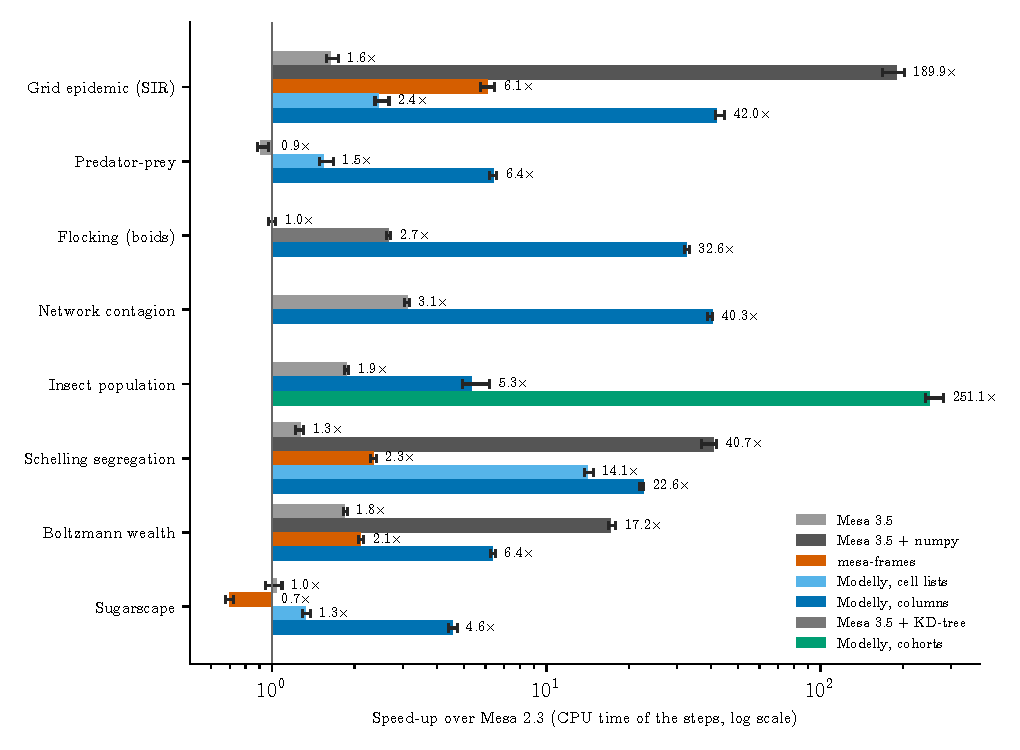
\includegraphics[width=\linewidth]{figures/speedups}
  \caption{$S_{\mathrm{steps}}$ of each implementation over the Mesa~2.3
  implementation of the same workload (\cref{tab:playbooks}); whiskers span the per-round
  ratios, and bars left of 1 are slower than Mesa~2.3. Columns and cohorts are \modelly{}'s
  array-based storage; cell lists keep per-cell agent lists, as Mesa's grids do; mesa-frames is the vectorised
  data-frame library built on Mesa; Mesa~3.5 + numpy replaces Mesa's agents with hand-written
  arrays.}
  \label{fig:speedups}
\end{figure}

\paragraph{Where \modelly{} is fast, and why.} \modelly{}'s column form runs every workload
faster than Mesa~2.3 and Mesa~3.5, and faster than mesa-frames on the four it implements
(\cref{tab:playbooks,fig:speedups}): its steps run
4.6 to 42 times faster than Mesa~2.3, 2.9 to 33 times faster than Mesa~3.5 and 3.0 to 9.6 times
faster than mesa-frames, and its cohort form runs the insect population 251 times faster than
Mesa~2.3 and 135 times faster than Mesa~3.5. \Cref{tab:why} gives the reason workload by
workload. In each, one \modelly{} mechanism replaces a Python loop over the agents with a few
array operations over the whole population: a column read or write instead of an attribute per
agent, one count over the grid's adjacency instead of a neighbourhood walk per agent, one
KD-tree query instead of a distance test per pair, one sparse product over a network instead of
a loop over each node's neighbours, one binomial draw per class instead of one draw per insect.
The gain therefore grows with the share of a step that such a mechanism covers: largest where
every phase becomes array work (flocking, the grid epidemic, Schelling's model, the network),
smaller where a phase must stay sequential, as the foragers' walk to a free cell in Sugarscape,
or where the step creates and removes many agents, as the births and deaths of predator-prey
and of the individual insect model, or where a cost every implementation shares dominates the
step, as Boltzmann wealth's data collector, which records the Gini coefficient and every
agent's wealth after each step (\cref{sec:threats}). Code that gives up agent objects
altogether goes further still: hand-written numpy is 1.8 to 4.5 times faster than the columns
(below). The arguments that each vectorised phase has the law of its
per-agent loop are given in the documentation (\code{docs/vectorised\_phases.md}), and
\cref{sec:agreement} checks that the outputs agree.

\begin{table}[tbp]
  \centering
  \small
  \caption{Where \modelly{}'s speed comes from: for each workload, from the largest step-time
  speed-up over Mesa~2.3 in \cref{tab:playbooks} to the smallest (the insect population by its
  cohort form), the mechanism that replaces the per-agent
  Python loop, as the code of each implementation shows (the attribution comes from the code,
  not from per-workload profiles).}
  \label{tab:why}
  \begin{tabularx}{\linewidth}{@{}l >{\raggedright\arraybackslash}X@{}}
    \toprule
    Workload & What \modelly{} does instead of a loop over agents \\
    \midrule
    Insect population & cohorts: at most about 190 (stage, age, sex) classes thinned by
      binomial draws replace about 26,000 agents \\
    Grid epidemic & positions are a column of cells: the walk is one \code{random\_neighbor}
      call, the exposure one count of infected per cell \\
    Network contagion & infected neighbours of every node in one sparse matrix--vector
      product; infection and recovery are Bernoulli vectors \\
    Flocking & one periodic KD-tree query for the whole flock; the steering terms are pair sums
      scattered back with \code{bincount}; positions written in one call \\
    Schelling & happiness is two sparse products (residents per cell, summed over neighbours);
      all moves in one pass with the sequential rule's law \\
    Predator-prey & movement, energy, grazing and predation (\code{claim}) are array
      operations; deaths and births are one call per species \\
    Boltzmann wealth & the exchange is a few array passes (a fixed-point iteration) with the
      law of the shuffled sequential order \\
    Sugarscape & every forager's best visible cell found in one array pass; only the walk to
      a free cell stays sequential \\
    \bottomrule
  \end{tabularx}
\end{table}

\paragraph{The other implementations.} Mesa~3.5 is faster than Mesa~2.3 on five workloads
(1.3 to 3.1 times), as fast on flocking and Sugarscape, and slower on predator-prey (0.91
times). mesa-frames is 2.1 to 6.1 times faster than Mesa~2.3 on three of its four workloads and
slower on Sugarscape (0.70 times), where its per-forager search is a cross join and a sort over
up to about 130,000 rows per step. \modelly{}'s cell-list variants, which keep per-cell
agent lists, give 1.3 to 14 times over Mesa~2.3 and 1.3 to 11 over Mesa~3.5: large for
Schelling's model, whose residents mostly count their neighbours, small where movement and
search stay per agent. Construction is where \modelly{} spends more than Mesa~2.3 (it
allocates the columns and indexes the space; Mesa~3.5's cell spaces cost about as much, 0.31
to 0.43~s on the three large grids and the network), so the column form's gain including construction is
4.0 to 32 times, and lower than per step on short runs such as the network contagion (40 times
per step, 10 in total).

\paragraph{Against hand-written numpy.} The Mesa~3.5 + numpy baseline is faster than
\modelly{}'s columns on all three of its workloads: its steps take 0.034~s against 0.155~s on
the grid epidemic (4.5 times faster, 95\% interval 4.1 to 4.6), 0.112~s against 0.201~s on
Schelling's model (1.8 times, 1.8 to 1.8) and 0.121~s against 0.328~s on Boltzmann wealth (2.7
times, 2.7 to 2.7; there partly because it records the wealth as one array per step rather than
as per-agent rows). It pays for that with the model's structure: no agent has an identity,
methods or attributes of its own, the population cannot hold agents of several kinds, every
neighbourhood is a hand-built index table, and every phase has to be rewritten as array
operations before the model runs at all, whereas \modelly{} keeps agent objects, agent sets and
spaces next to the columns, and lets a model be vectorised one phase at a time. Its agreement
with Mesa~2.3 is that of the other implementations (\cref{tab:agreement-mesa3np}: 13 of 14
statistics equivalent within $0.5\,s_p$); the one paired $t$-test below 5\% after the Holm
correction is Schelling's segregation ($d = 0.24$, 0.6\% of the mean). The baseline runs the
column algorithm without the framework layer, and on these seeds its Schelling and Boltzmann
wealth runs give exactly the column variant's statistics, so the two share this difference
and any bias behind it; on 300 new seeds the column variant's segregation has $d = 0.07$
$[-0.02, 0.15]$ (\cref{tab:agreement-schelling300}). The benchmark harness's own six-seed
check flags three of its six grid epidemic statistics, flags that vanish over 100 seeds (at the
small size lowest paired $p$ 0.13 and largest $|d|$ 0.21; at the timed size 0.19 and 0.20;
all six equivalent in both; \code{paper/data/agreement\_large\_grid\_mesa3np.json}). The gap is the price of the
framework layer: \modelly{} sits between per-agent Mesa and hand-written arrays,
3.5 to 26 times above Mesa~3.5 and 1.8 to 4.5 times below the numpy baseline on these three workloads.

\paragraph{How the gain changes with population size.} The playbooks are timed at one size;
\cref{tab:sizes} times three of them, whose populations scale with one parameter, at the
playbook's small size, its timed size and ten times that, five rounds each on the same
fixed-frequency core (\code{paper/scripts/sizes.py}, \code{paper/data/sizes.json}). On the
grid epidemic and Schelling's model the columns' lead grows with the population: on the grid
epidemic it goes from 4.0 to 42 and 119
times over Mesa~2.3 and from 2.4 to 26 and 67 times over Mesa~3.5 as the population goes from
2,000 to 20,000 and 200,000 agents; on Schelling's model from 1.3 to 22 and 44 times over
Mesa~2.3 and from 1.0 to 18 and 32 times over Mesa~3.5; on Boltzmann wealth, whose data
collector records every agent's wealth each step, it grows over Mesa~2.3 (4.0, 6.4 and 10
times) but stays at 2.8 to 3.6 times over Mesa~3.5, and shrinks over mesa-frames (14, 3.0 and
2.0 times). At the smallest sizes the framework's fixed cost per step weighs most: on Schelling's model with
1,282 residents the columns are as fast as Mesa~3.5. Hand-written numpy's lead over the columns
shrinks the other way on the grid epidemic (17, 4.6 and 1.6 times) and Schelling's model (13.5,
1.8 and 1.0 times), where at large populations the columns run at nearly the speed of code
without agents while keeping them; on Boltzmann wealth it stays at 1.9 to 2.8 times.

\begin{table}[tbp]
  \centering
  \small
  \caption{The step-time speed-ups of \modelly{}'s columns, and of hand-written numpy over the
  columns, at three population sizes: the playbook's small size, its timed size (as in
  \cref{tab:playbooks}) and ten times that at the same density. Medians of five rotated rounds
  on one fixed-frequency core; agents at the end of the run. Generated by
  \code{paper/scripts/sizes.py}.}
  \label{tab:sizes}
  \setlength{\tabcolsep}{4pt}
  \begin{tabular}{llrrrrrr}
\toprule
 & & & & \multicolumn{3}{c}{columns faster than} & numpy faster \\ \cmidrule(lr){5-7} Workload & Size & Agents & Mesa 2.3, s & Mesa 2.3 & Mesa 3.5 & mesa-frames & than columns \\
\midrule
Grid epidemic & small & 2{,}000 & 0.40 & 4.0 & 2.4 & 2.6 & 17.0 \\
 & large & 20{,}000 & 6.50 & 42.2 & 25.9 & 6.9 & 4.6 \\
 & huge & 200{,}000 & 95.49 & 119 & 66.6 & 12.6 & 1.6 \\
\addlinespace
Schelling & small & 1{,}282 & 0.13 & 1.3 & 1.0 & 2.6 & 13.5 \\
 & large & 32{,}090 & 4.50 & 22.4 & 17.9 & 9.6 & 1.8 \\
 & huge & 319{,}610 & 58.69 & 43.9 & 32.1 & 16.9 & 1.0 \\
\addlinespace
Boltzmann wealth & small & 500 & 0.08 & 4.0 & 2.8 & 14.1 & 1.9 \\
 & large & 10{,}000 & 2.10 & 6.4 & 3.5 & 3.0 & 2.7 \\
 & huge & 100{,}000 & 41.33 & 10.2 & 3.6 & 2.0 & 2.8 \\
\bottomrule
\end{tabular}

\end{table}

\paragraph{On other interpreters.}
\label{sec:python-versions}
Every timing above ran on CPython~3.15. Since per-agent code gains from each interpreter
release and array code does not, the ratios could depend on the version, so we timed the
Mesa~3.5 and column implementations of all eight playbooks (and the insect population's
cohorts) under CPython 3.12, 3.14 and 3.15, each in its own environment with the same
package versions and \modelly{}'s C modules built for it, five rotated rounds in fresh
interpreters pinned to one core at the machine's default frequency policy
(\code{paper/scripts/python\_versions.py}, \cref{tab:python-versions} in the appendix). The
speed-ups on 3.15 reproduce \cref{tab:playbooks}'s within the session's noise (26.1, 7.1,
31.5, 12.9, 3.0, 17.7, 3.5 and 4.4 against 25.7, 7.1, 32.6, 12.9, 2.9, 17.8, 3.5 and 4.4;
the cohorts 135 against 135), and on 3.12 and 3.14 they are similar or larger: 33 and 32
on the grid epidemic, 9.7 and 7.7 on predator-prey, 17 and 22 on Schelling's model, 4.3 and
4.2 on Boltzmann wealth, within 10\% of the 3.15 values on the other four, with the
cohorts at 151 and 159. Mesa's per-agent steps are 1 to 28\% faster on 3.15 than on 3.12
(20\% on the grid epidemic, 28\% on predator-prey) while the columns' steps change by at
most 5\% on six playbooks (16\% on Schelling's model and 14\% on the insect population,
whose column steps keep some per-agent work), so the newest interpreter is the least
favourable of the three to \modelly{} on six of the eight workloads (a tie on the insect
population's columns; Schelling's model 5\% lower on 3.12), and the speed-ups reported in
the paper are, within 5\%, the conservative ones.

\paragraph{A sweep end to end.}
\label{sec:sweep}
Step time dominates long runs; a sweep of short runs also pays for starting workers,
importing and building the model, reading its outputs after every step and writing them
to the store. We timed one small sweep end to end (\code{paper/scripts/sweep\_e2e.py},
\cref{tab:sweep} in the appendix): 64 runs of the grid epidemic at the small size (a
16-point Latin hypercube over $\beta$, four replicates, 60 steps, one output per step), from
the creation of the \code{Experiment} to its results queried from the Parquet store,
driven by \modelly{}'s experiment layer with each of the two engines, the column
implementation and the Mesa~3.5 one (which takes its parameters by name and steps like any
model, so the workflow's overhead is the same on both sides), medians of five rounds in
fresh interpreters. On the serial executor pinned to one core the sweep takes 2.18~s with
the columns and 16.98~s with Mesa~3.5, a factor of 7.8, against 12 for the simulation alone
at this size (0.020 against 0.244~s per run): with runs this short, 40\% of the column
sweep is the workflow (0.014~s per run: the task's dispatch, the output read after each of
the 61 states, the Parquet write) and 8\% of the Mesa one. On four processes the Mesa sweep is 2.4 times faster than serial and
the column sweep no faster (2.20~s): 64 runs of 0.02~s do not repay starting four workers
and importing the model in each, so a sweep of runs this short on \modelly{} should stay
serial, or batch many runs per task. The gain a study sees from the columns is therefore
the step-time speed-up for long runs and, for short runs, a smaller factor that the
workflow's fixed cost per run bounds; \cref{tab:playbooks}'s $S_{\mathrm{total}}$ gives
the bound from construction alone, and this measurement adds the experiment layer's share.
The session ran at the machine's default frequency policy under a load average of 10 to 21
(the fourth round, under the heaviest load, is the slowest in every arm).

\paragraph{mesa-frames with more threads.} polars runs multi-threaded by default, while the
timings above set \code{POLARS\_MAX\_THREADS=1} so that every implementation uses one core;
pinned to the four performance cores, five alternating rounds in wall-clock time, mesa-frames
with four threads was slower than with one on all four of its workloads (Schelling's model
3.41~s against 2.86~s; \code{paper/data/frames\_threads\_pinned.json}), so on those cores the
one-thread comparison does not handicap it. With all 16 threads, unpinned, single runs gave
Schelling's model 1.4 times faster and the other three slower (\cref{app:workloads}): on the
whole machine the one-thread comparison may overstate the columns' lead on Schelling's model
by up to that factor.

\subsection{Where the gain comes from: an ablation}
\label{sec:ablation}

Between per-agent Mesa~3.5 code and \modelly{}'s column form several things change at
once: the framework whose calls the same code makes, whether those calls run in C or in
Python, the data structure that holds the population, the algorithm of a search, and
whether a phase is written per agent or as array operations. To attribute the gain, we timed
a ladder of implementations that changes one of these per rung on four workloads
(\code{paper/scripts/ablation.py}, \cref{tab:ablation}): ten rotated rounds in fresh
interpreters pinned to one core, each \modelly{} rung run twice, once with
\code{MODELLY\_PURE\_PYTHON=1} (the framework's inner loops in Python) and once with the C
modules, so that the compiled runtime's share is read off within the rung. The session ran
at the machine's default frequency policy, so its absolute times differ from
\cref{tab:playbooks} (they are 6 to 19\% shorter); every ratio is paired within the
session, and the speed-ups of the columns over Mesa~3.5 that it gives (26.4, 18.5, 33.5
and 4.5) agree with the main table's (25.7, 17.8, 32.6 and 4.4) within 4\%.

\begin{table}[htbp]
  \centering
  \small
  \caption{The ablation: one ladder of implementations per workload, each rung changing one
  thing from the rung above. Median CPU time of the steps over ten rotated rounds with the
  framework's inner loops in Python (\code{MODELLY\_PURE\_PYTHON=1}) and compiled; the
  compiled runtime's gain within the rung (median of the per-round ratios); and the speed-up
  of the compiled rung over Mesa~3.5 and over the rung above. The Mesa~3.5 and numpy rungs
  have no Python-core arm. Generated by \code{paper/scripts/ablation.py} from
  \code{paper/data/ablation.json}.}
  \label{tab:ablation}
  \setlength{\tabcolsep}{4pt}
  \begin{tabularx}{\linewidth}{l>{\raggedright\arraybackslash}Xrrrrr}
\toprule
 & & \multicolumn{2}{c}{steps (s)} & & \multicolumn{2}{c}{speed-up (compiled)} \\
\cmidrule(lr){3-4}\cmidrule(lr){6-7}
Workload & Rung & Python & compiled & C gain & Mesa~3.5 & rung above \\
\midrule
Grid epidemic & Mesa 3.5: per-agent code on Mesa's cell space & -- & 3.526 & -- & 1.0 & -- \\
 & migrated: same code, Modelly's calls (codemod) & 3.284 & 2.627 & 1.27 & 1.3 & 1.34 \\
 & cell lists: Mesa's data structure; infection phase as arrays & 2.880 & 2.328 & 1.23 & 1.5 & 1.10 \\
 & columns: every phase as arrays over columns & 0.131 & 0.133 & 0.99 & 26.4 & 18.00 \\
 & Mesa 3.5 + numpy: arrays without agent objects or framework & -- & 0.029 & -- & 119.1 & 4.56 \\
\addlinespace
Schelling & Mesa 3.5: per-agent code on Mesa's cell space & -- & 3.367 & -- & 1.0 & -- \\
 & migrated: same code, Modelly's calls (codemod) & 3.239 & 3.110 & 1.04 & 1.1 & 1.10 \\
 & cell lists: Mesa's data structure; neighbour count as arrays & 0.330 & 0.302 & 1.09 & 11.3 & 10.08 \\
 & columns: every phase as arrays over columns & 0.180 & 0.183 & 1.00 & 18.5 & 1.65 \\
 & Mesa 3.5 + numpy: arrays without agent objects or framework & -- & 0.105 & -- & 32.7 & 1.73 \\
\addlinespace
Flocking & Mesa 3.5: per-agent code, all-pairs neighbour scan & -- & 23.039 & -- & 1.0 & -- \\
 & Mesa 3.5 + KD-tree: same code, one KD-tree per step & -- & 8.335 & -- & 2.6 & 2.60 \\
 & columns: KD-tree; steering as arrays over columns & 0.668 & 0.663 & 1.04 & 33.5 & 13.15 \\
\addlinespace
Sugarscape & Mesa 3.5: per-agent code, one search per forager & -- & 1.158 & -- & 1.0 & -- \\
 & cell lists: Mesa's data structure, same search & 0.994 & 0.909 & 1.10 & 1.3 & 1.25 \\
 & columns: search as one array pass over columns & 0.260 & 0.257 & 1.00 & 4.5 & 3.50 \\
\bottomrule
\end{tabularx}
% 10 rounds, core 2

\end{table}

\paragraph{What each rung contributes.} The framework's own calls, with no phase rewritten,
are worth little: the same code migrated to \modelly{} runs 1.06 times faster than on
Mesa~3.5 with the inner loops in Python (grid epidemic and Schelling alike), and the C
modules add a factor of 1.27 on the grid epidemic, whose step is dominated by per-agent
moves and neighbourhood reads that the compiled loops serve, and 1.04 on Schelling's model,
whose step is dominated by neighbour counting in model code. The data structure alone is
worth about as little: on Sugarscape, where the cell-list variant runs Mesa's search
algorithm on \modelly{}'s cell lists, it gives 1.13 with the Python core and 1.25 with the
compiled one. The algorithm is worth what it is worth: the KD-tree alone makes Mesa~3.5's
flocking 2.6 times faster. Everything else is the array form of the phases. On the grid
epidemic, moving from cell lists to columns, with no change of algorithm and with the C
modules off on both sides, is a factor of 22; on Schelling's model vectorising the
neighbour count alone (the cell-list rung, Python core) is a factor of 10 over the migrated
code and vectorising the moves as well (columns) another 1.8; on flocking the steering
terms as array operations are a factor of 12.5 over the KD-tree baseline; on Sugarscape
the search as one array pass is a factor of 3.9 over the same search per forager. The
compiled runtime contributes nothing to the column rungs (0.99 to 1.04): once a phase is an
array operation, the framework's loops are no longer on the path, and the time is numpy's.
In the ablation's session the column form sits 1.7 to 4.6 times above hand-written numpy
without agent objects (1.8 to 4.5 in \cref{tab:playbooks}),
which is the price of keeping agents, agent sets and spaces next to the arrays.
The attribution is therefore: of the grid epidemic's factor of 26, about 1.3 is the
framework and its compiled loops and about 20 the array representation of the phases; of
flocking's 34, 2.6 is the neighbour-search algorithm and 13 the array form of the
steering; of Schelling's 19, 1.1 is the framework and 17 the array form; of Sugarscape's
4.5, 1.25 is the data structure and 3.5 the array form of the search.

\subsection{Do the faster forms compute the same model?}
\label{sec:agreement}

The implementations draw their random numbers in different orders, so their dynamics cannot
agree run by run; they must agree in distribution. Where two implementations draw the initial
state the same way, a seed gives both the same start: strongly in Sugarscape (correlation
between the two implementations' outputs on a seed $r = 0.91$ to $0.99$) and Schelling's model
($0.42$ to $0.70$), completely in flocking, whose dynamics are deterministic once it has
started ($r = 1$). The comparisons are therefore paired, seed by seed. We ran the Mesa~2.3
reference and every \modelly{} variant of every playbook on the same 100 seeds at the playbook's
small size (2,100 runs), and compared each of the 67 pairs of a summary statistic and a \modelly{} variant (epidemic peak
and final size, final populations, cluster counts, Gini coefficient, and so on) with the Mesa
reference in three ways: a paired $t$-test on the seed-by-seed differences, the two-sample
Kolmogorov--Smirnov test on the two marginal distributions (an unpaired test, conservative
here because the shared seeds correlate the samples, and more so for the integer-valued
statistics, whose values tie, so it serves as a coarse check only), and paired two one-sided tests
(TOST) of equivalence \citep{schuirmann1987comparison, lakens2017equivalence} with a margin of
half a pooled standard deviation $s_p$, that is, against the null hypothesis
$|\mu_{\mathrm{Modelly}} - \mu_{\mathrm{Mesa}}| \ge 0.5\, s_p$. We report the standardised
difference $d = (\bar x_{\mathrm{Modelly}} - \bar x_{\mathrm{Mesa}}) / s_p$ with its paired 95\%
interval, and correct for the 67 comparisons with Holm's procedure \citep{holm1979simple}.
\Cref{tab:agreement-all} in the appendix lists every comparison. Three kinds of statement
follow from these tests, and we keep them apart throughout: a comparison is \emph{shown
equivalent} when its TOST rejects at 5\% (nominally, one comparison at a time; or after the
Holm correction, which controls the familywise error over the 67); a comparison is
\emph{shown different} when its paired interval excludes zero; and a comparison that is
neither is \emph{undecided}, not equal, since a nonsignificant difference test can reflect
low power. The margin of $0.5\,s_p$ is a convention (a medium effect by Cohen's scale), not
a scientific tolerance; we therefore also report how the counts change with the margin,
give counts at margins relative to Mesa's mean, and, in \cref{sec:trajectories}, test
science-specific margins prespecified in each quantity's own units.

\begin{table}[htbp]
  \centering
  \small
  \caption{Agreement with Mesa~2.3 over 100 shared seeds per variant, at the small size: the
  largest standardised difference, the lowest paired $t$ and Kolmogorov--Smirnov $p$-values
  (before correction), and the number of statistics equivalent within $0.5\,s_p$ (paired TOST
  at 5\%, uncorrected).
  Generated by \code{paper/scripts/agreement.py}.}
  \label{tab:agreement}
  \begin{tabular}{llrrrrr}
\toprule
Workload & Modelly variant & Stats & max $|d|$ & min $p_{t}$ & min $p_{\mathrm{KS}}$ & Equivalent \\
\midrule
Grid epidemic & cell lists & 6 & 0.23 & 0.08 & 0.15 & 6/6 \\
Grid epidemic & columns & 6 & 0.13 & 0.39 & 0.58 & 6/6 \\
Predator-prey & cell lists & 5 & 0.30 & 0.02 & 0.01 & 4/5 \\
Predator-prey & columns & 5 & 0.13 & 0.34 & 0.47 & 5/5 \\
Flocking & columns & 3 & 0.00 & 0.90 & 1.00 & 3/3 \\
Network contagion & columns & 6 & 0.16 & 0.20 & 0.21 & 6/6 \\
Insect population & columns & 6 & 0.33 & 0.02 & 0.04 & 4/6 \\
Insect population & cohorts & 6 & 0.23 & 0.10 & 0.21 & 6/6 \\
Schelling & cell lists & 4 & 0.23 & 0.03 & 0.37 & 4/4 \\
Schelling & columns & 4 & 0.24 & $<$0.01 & 0.28 & 4/4 \\
Boltzmann wealth & columns & 4 & 0.29 & 0.03 & 0.21 & 3/4 \\
Sugarscape & cell lists & 6 & 0.03 & 0.33 & 0.82 & 6/6 \\
Sugarscape & columns & 6 & 0.01 & 0.65 & 0.97 & 6/6 \\
\bottomrule
\end{tabular}
% 100 seeds per variant

\end{table}

\begin{figure}[htbp]
  \centering
  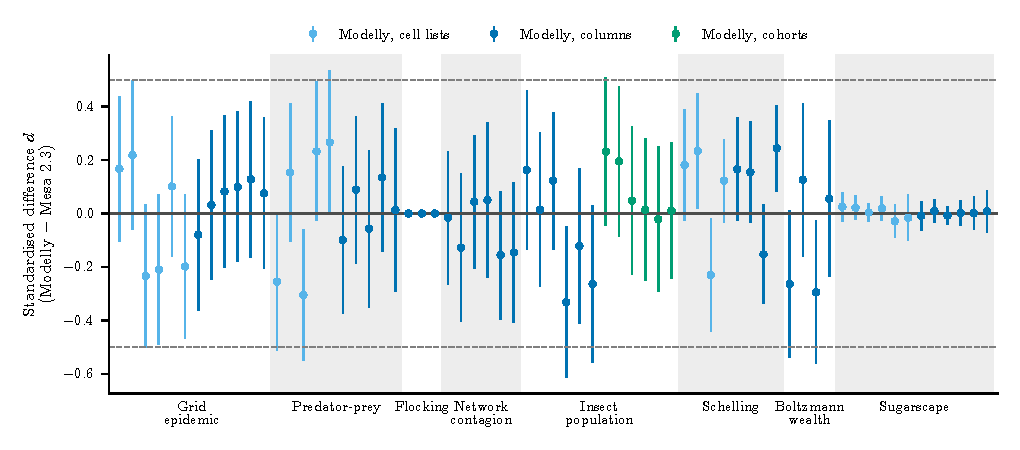
\includegraphics[width=\linewidth]{figures/agreement_small}
  \caption{Standardised difference $d$ between each \modelly{} variant and Mesa~2.3 for every
  summary statistic, with 95\% intervals, over 100 seeds; dashed lines: the equivalence margin
  $\pm 0.5\,s_p$. Flocking is deterministic once its initial state is drawn, and both
  implementations draw it from the same seeded \code{numpy} stream: it agrees run by run to
  rounding error, hence $d = 0$.}
  \label{fig:agreement}
\end{figure}

\Cref{tab:agreement} and \cref{fig:agreement} give the results. Within the margin of
$0.5\,s_p$, 63 of the 67 comparisons are shown equivalent at the nominal 5\% level (60 of 64
outside flocking, whose three agree trivially), and 29 of 67 after the Holm correction of
the TOST $p$-values. The two counts answer different questions: the first says how many
comparisons, each taken on its own, meet the margin; the second how many do so with the
familywise error held at 5\% over all 67, and it is the one to quote when the claim is
about the set. The four comparisons not shown equivalent even nominally are the mean sheep
population of predator-prey with cell lists, the final and the peak adult counts of the
individual insect model, and the share of agents without wealth in the Boltzmann model
($|d| \le 0.33$, at most 1.4\% of the mean). The count depends on the margin: 50 at
$0.4\,s_p$, 27 at $0.3\,s_p$ and 19 at $0.25\,s_p$; with a margin relative to Mesa's mean
instead, 48 of 67 are shown equivalent within $\pm 5\%$ and 56 within $\pm 10\%$, the others
being the noisiest statistics at this small size (the grid epidemic's counts with 2,000
agents, predator-prey's wolves), whose 100-seed intervals are wider than those margins.
The intervals themselves are the most direct summary: every $|d|$ is at most 0.33, 58 of the 67 intervals lie within $[-0.5, 0.5]$ and all
within $[-0.62, 0.62]$; every difference of means is at most 11\% of Mesa's, and under 5\%
for 59 of 67. Six intervals exclude zero, so six differences are shown,
taken one at a time: three in Schelling's model ($|d| \le 0.24$, at most 4.3\% of the
mean, made detectable by the shared initial state), the mean sheep population of
predator-prey with cell lists, the final adult count of the individual insect model and the
share of agents without wealth in the Boltzmann model ($|d| \le 0.33$, at most 1.4\%).
After the Holm correction no paired or Kolmogorov--Smirnov test falls below 5\% (the
smallest corrected paired $p$ is 0.21); we do not read this as equality, since at the
corrected level a paired test on 100 seeds detects $d = 0.33$ with probability 0.13 only
(\cref{sec:threats}), but as consistent with the intervals above. Before correction, six
paired $t$-tests and three Kolmogorov--Smirnov tests fall below 5\%, against 3.2 expected by
chance for each test among the 64 comparisons outside flocking if the tests were
independent (they are not: the statistics of a workload are related, such as its final S, I
and R). The spreads agree too: the ratio of the two implementations' standard deviations
lies between 0.77 and 1.27, and one median-centred Levene test \citep{brown1974robust} of 67
falls below 5\%, none after the Holm correction; within the power of a Levene test on 100
seeds (unpaired, and so conservative here) this is consistent with a vectorised phase
leaving the variability of an outcome unchanged, and no more. The benchmark harness's own
quick check, six seeds and an unpaired Welch test \citep{welch1947generalization} at 1\%,
could not have shown any of this: its power to detect a difference of one standard
deviation is 13\%.

\paragraph{At the timed size.} We repeated the study at the large size used for the timings,
with 50 seeds per variant (1,050 runs; \cref{tab:agreement-large}). 53 of the 67
comparisons are shown equivalent within the margin (nominally), fewer than at the small
size because half as many seeds give wider intervals; one paired $t$-test (Sugarscape with
cell lists, mean wealth, $d = 0.11$, 0.3\% of the mean) and two Kolmogorov--Smirnov tests
fall below 5\% before the Holm correction and none after it, with the caveat on power
above. The largest differences were in the grid epidemic's peak time, about 11\% later in
both \modelly{} variants ($d = 0.43$ and $0.40$, paired $p = 0.05$ and $0.07$). A
replication on 200 new seeds, disjoint from these 50, does not reproduce them: no interval
of the twelve grid epidemic comparisons excludes zero, the largest $|d|$ is 0.13 (the peak
time's is 0.03 and 0.04, under 1\% of the mean), and all twelve are equivalent within
$0.4\,s_p$, also after the Holm correction. The trajectory study at the small size
(\cref{sec:trajectories}) finds the columns' peak 3.3 steps \emph{earlier} on 100
other seeds; taken together, the three samples put the columns' peak timing within about
$\pm 12\%$ of Mesa's, with the sign undetermined, which is what the tests' power at this
margin allows.

\paragraph{The other baselines against Mesa~2.3.} The same study on the Mesa~3.5 and
mesa-frames implementations (100 seeds at the small size, 2,000 runs;
\cref{tab:agreement-baselines}) finds all 40 Mesa~3.5 statistics equivalent within
$0.5\,s_p$ with nothing below 5\% even before correction, and 18 of the 20 mesa-frames
statistics equivalent with one difference that survives the Holm correction ($p = 0.013$):
its Schelling implementation ends more segregated than Mesa~2.3's ($d = 0.31$, 0.7\% of the
mean). A replication of Schelling's model on 300 new seeds (\cref{tab:agreement-schelling300})
finds no difference after the Holm correction for any implementation; before it, mesa-frames'
segregation still differs ($d = 0.10$ $[0.01, 0.18]$, 0.2\% of the mean, $p = 0.02$), as do
Mesa~3.5's share of happy residents and number of moves ($|d| \le 0.23$, at most 3.8\%),
while neither \modelly{} variant does. The mesa-frames shift is small, its cause in our
implementation unknown, and it does not change its timing's order of magnitude.
\Cref{tab:agreement-grid200} gives the grid epidemic over 200 new seeds.

\begin{table}[htbp]
  \centering
  \small
  \caption{As \cref{tab:agreement}, at the large size of the timings, over 50 shared seeds per
  variant.}
  \label{tab:agreement-large}
  \begin{tabular}{llrrrrr}
\toprule
Workload & Modelly variant & Stats & max $|d|$ & min $p_{t}$ & min $p_{\mathrm{KS}}$ & Equivalent \\
\midrule
Grid epidemic & cell lists & 6 & 0.43 & 0.05 & 0.04 & 2/6 \\
Grid epidemic & columns & 6 & 0.40 & 0.07 & 0.07 & 4/6 \\
Predator-prey & cell lists & 5 & 0.21 & 0.25 & 0.27 & 4/5 \\
Predator-prey & columns & 5 & 0.14 & 0.41 & 0.27 & 5/5 \\
Flocking & columns & 3 & 0.00 & 0.22 & 1.00 & 3/3 \\
Network contagion & columns & 6 & 0.27 & 0.14 & 0.18 & 5/6 \\
Insect population & columns & 6 & 0.33 & 0.12 & 0.02 & 3/6 \\
Insect population & cohorts & 6 & 0.20 & 0.31 & 0.18 & 4/6 \\
Schelling & cell lists & 4 & 0.09 & 0.46 & 0.72 & 4/4 \\
Schelling & columns & 4 & 0.07 & 0.59 & 0.72 & 4/4 \\
Boltzmann wealth & columns & 4 & 0.19 & 0.37 & 0.27 & 3/4 \\
Sugarscape & cell lists & 6 & 0.11 & 0.02 & 0.55 & 6/6 \\
Sugarscape & columns & 6 & 0.07 & 0.06 & 0.72 & 6/6 \\
\bottomrule
\end{tabular}
% 50 seeds per variant

\end{table}

\subsection{Do the faster forms follow the same dynamics?}
\label{sec:trajectories}

Summary statistics at the end of a run can agree while the runs that produce them differ:
in the shape of the epidemic curve, the spatial pattern it leaves, the speed at which a city
segregates, the period of a predator-prey cycle, or how often a species dies out. We
therefore compared trajectories and patterns on three playbooks, over 100 new shared seeds
(20,000 to 20,099, disjoint from the playbook studies' seeds) at the small size, each \modelly{}
variant against Mesa~2.3, and, as a reference for what two per-agent implementations of
the same model differ by, Mesa~3.5 against Mesa~2.3 on the same seeds
(\code{paper/scripts/trajectories.py}). The quantities and their margins were fixed before
the runs (\cref{tab:trajectories-all} lists them): for the grid epidemic, the whole
infected curve, the peak's height and timing, the final size, and the clusters of cells with
anyone ever infected at the end (8-connected on the torus: their number, the largest and
the mean size); for Schelling's model, the curves of the happy share and of the moves, the
final segregation and happy share, the composition of every resident's neighbourhood (the
share of residents in each of ten bins of the same-kind share), and the time to converge
(steps with moves above 2\% of the residents); for predator-prey, run for 2,000 steps
rather than the playbook's 200 so that the cycle shows, the sheep, wolf and bare-grass
curves, the probability that the wolves or the sheep die out within the run, and the
amplitude and period of the sheep cycle (the first peak of its autocorrelation). The
margins are in each quantity's own units: 2 steps for a timing, 0.02 for a share, 5
percentage points for a probability, $\pm 5\%$ of Mesa's mean for a count the primary study
already covers and $\pm 10\%$ for a derived quantity. Each scalar is tested by a paired TOST at
its margin, the 78 scalars Holm-corrected as one family; each curve by the largest
standardised difference over its steps, $\sup_t |d_t|$, with a 95\% upper bound from a
bootstrap over seeds, and by a sign-flip permutation test of the same statistic.

\begin{table}[htbp]
  \centering
  \small
  \caption{Trajectories and patterns over 100 shared seeds at the small size: per workload
  and implementation, the number of curves compared, the largest standardised difference
  over all steps of any curve and its 95\% bootstrap upper bound, the number of scalar
  quantities, their largest $|d|$, and how many are shown equivalent at their prespecified
  margin (paired TOST at 5\%; in brackets, after the Holm correction over all 78 scalars).
  Mesa~3.5 against Mesa~2.3 is the reference: two per-agent implementations of the same
  model. Generated by \code{paper/scripts/trajectories.py}; \cref{tab:trajectories-curves,tab:trajectories-all} in the
  appendix give every curve and every scalar.}
  \label{tab:trajectories}
  \begin{tabular}{llrrrrrr}
\toprule
Workload & Implementation & Curves & $\sup_t |d_t|$ & upper 95\% & Scalars & max $|d|$ & Equivalent \\
\midrule
Grid epidemic & Mesa 3.5 & 1 & 0.15 & 0.46 & 6 & 0.18 & 2/6 (2) \\
Grid epidemic & cell lists & 1 & 0.24 & 0.52 & 6 & 0.23 & 2/6 (2) \\
Grid epidemic & columns & 1 & 0.34 & 0.54 & 6 & 0.28 & 2/6 (2) \\
Schelling & Mesa 3.5 & 2 & 0.13 & 0.46 & 14 & 0.17 & 13/14 (11) \\
Schelling & cell lists & 2 & 0.28 & 0.48 & 14 & 0.21 & 13/14 (12) \\
Schelling & columns & 2 & 0.07 & 0.29 & 14 & 0.18 & 14/14 (12) \\
Predator-prey & Mesa 3.5 & 3 & 0.39 & 0.67 & 6 & 0.15 & 5/6 (4) \\
Predator-prey & cell lists & 3 & 0.37 & 0.66 & 6 & 0.19 & 5/6 (3) \\
Predator-prey & columns & 3 & 0.35 & 0.65 & 6 & 0.14 & 5/6 (3) \\
\bottomrule
\end{tabular}
% 100 seeds per variant

\end{table}

\begin{figure}[htbp]
  \centering
  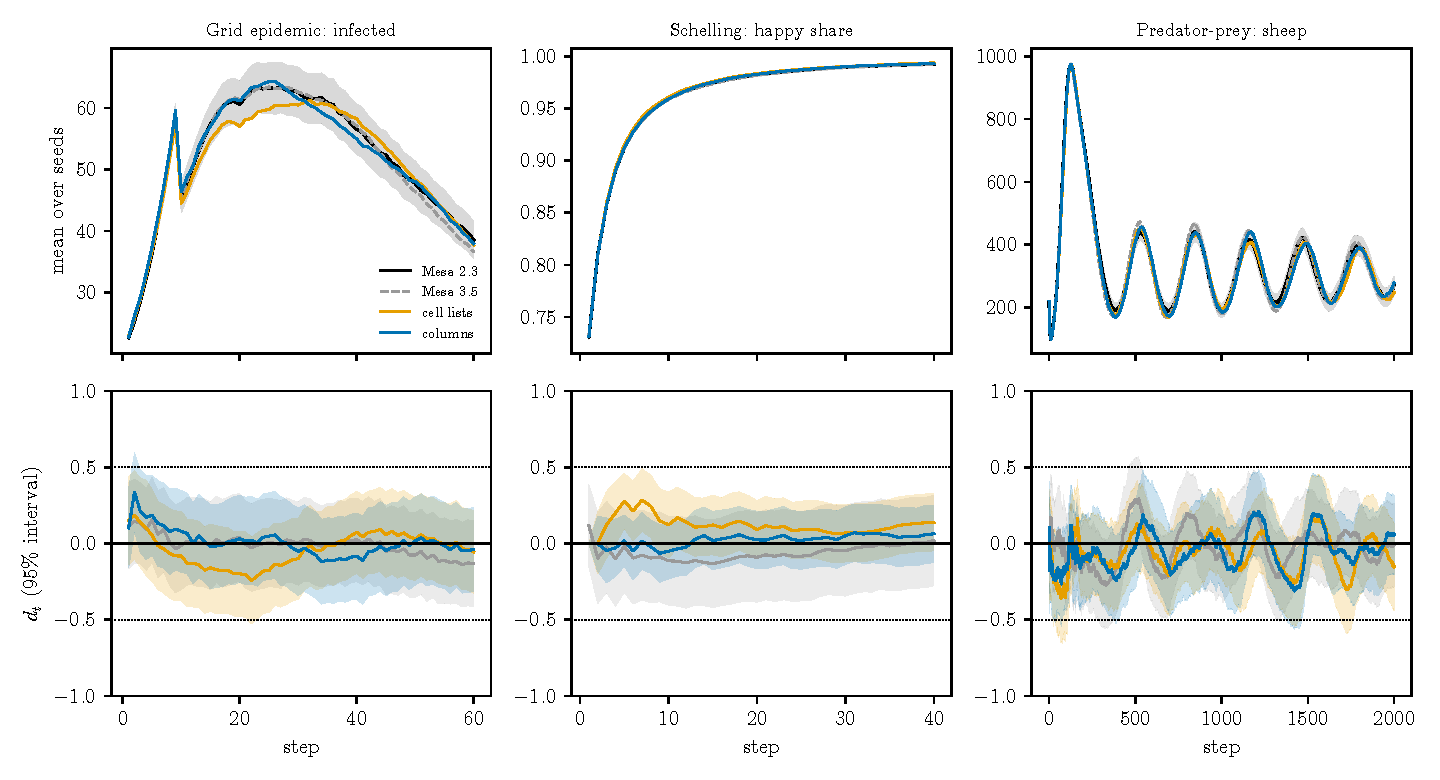
\includegraphics[width=\linewidth]{figures/trajectories_small}
  \caption{Top: the mean over 100 seeds of the infected count (grid epidemic), the happy
  share (Schelling) and the sheep count (predator-prey, 2,000 steps) for Mesa~2.3 (black,
  with a band of two standard errors), Mesa~3.5 (dashed) and the two \modelly{} variants.
  Bottom: the standardised paired difference $d_t$ from Mesa~2.3 at every step, with its
  95\% interval; dotted lines at $\pm 0.5$.}
  \label{fig:trajectories}
\end{figure}

\Cref{tab:trajectories} and \cref{fig:trajectories} give the results. On the curves, the
\modelly{} variants are as close to Mesa~2.3 as Mesa~3.5 is. On the grid epidemic's
infected curve the largest $|d_t|$ is 0.34 for the columns, 0.24 for the cell lists and
0.15 for Mesa~3.5 (upper bounds 0.54, 0.52 and 0.46), the largest relative difference of
the means over the steps where the epidemic is at least a tenth of its peak is 3.9, 7.4
and 5.3\%, one step of 60 has an interval excluding zero (the columns, at step 2, where
the first infections of the run are drawn), and no
permutation test finds a difference ($p = 0.16$, $0.52$, $0.92$). On Schelling's model the
columns follow Mesa~2.3 more closely than Mesa~3.5 does ($\sup_t |d_t| = 0.07$, upper
bound 0.29, against 0.13 and 0.46; the means of the happy share differ by at most 0.1\%)
while the cell lists show a small difference at steps 5 to 8 ($\sup_t |d_t| = 0.28$,
four steps with intervals excluding zero, permutation $p = 0.045$ for the happy share and
$0.048$ for the moves; at most 0.4\% of the happy share and 4.8\% of the moves). Over the
2,000 steps of predator-prey the largest $|d_t|$ is 0.29 to 0.39 for every implementation,
Mesa~3.5 included (upper bounds 0.61 to 0.67; a maximum over 2,000 noisy steps), the
permutation tests find nothing ($p \ge 0.24$), and the cycles of the four implementations
are in phase for 2,000 steps (\cref{fig:trajectories}): the same initial conditions set
the phase, and the period, 345 steps in Mesa~2.3, differs by at most 18 steps in the
others, with intervals of about $\pm 33$ steps.

On the scalars, 41 of the 52 \modelly{} comparisons are shown equivalent at their
prespecified margin (34 after the Holm correction) against 20 of 26 for Mesa~3.5 (17); the
study therefore does not establish equivalence for every quantity it tests, and we do not
claim that it does: 18 of the 52 are undecided at the familywise level. The
largest $|d|$ is 0.28 (Mesa~3.5: 0.18), and two paired $t$-tests of 52 fall below 5\% before
correction (none after; Mesa~3.5: none). The quantities not shown equivalent are the same
for every implementation, Mesa~3.5 included, and for the same reason: their margins are
narrower than what 100 seeds resolve. The peak's timing has a standard deviation of about
11 steps across seeds, so its paired interval is about $\pm 3.2$ steps against a margin of
$\pm 2$; the peak's height ($\pm 5\% = 3.8$ against an interval of $\pm 5.3$), the final
size ($\pm 14.6$ against $\pm 20$), the largest cluster ($\pm 1.9$ against $\pm 2.7$), the
total moves ($\pm 99$ against $\pm 110$, shown equivalent for the columns only) and the
period ($\pm 35$ against $\pm 33$) are the others. For all of these the point estimate lies
inside the margin, except the columns' peak timing, which is the one scalar shown different:
the columns' epidemic peaks $3.3$ steps earlier than Mesa~2.3's ($[-6.6, -0.1]$, $d =
-0.28$, 12\% of a mean of 28 steps); the cell lists' and Mesa~3.5's peak 2.9 and 2.1 steps
earlier with intervals that include zero. The second uncorrected difference is the cell
lists' share of residents with no same-kind neighbour, 0.4\% against 0.5\% ($d = -0.21$).
What the study does establish is this. Everything it was designed to catch beyond the
summary statistics agrees: the
cluster counts and mean cluster sizes are equivalent within $\pm 10\%$ for every
implementation after the Holm correction, the ten composition bins are equivalent within
0.02 for both \modelly{} variants before and after it (nine of ten for Mesa~3.5 after it),
the time to converge within 2 steps for every implementation before it, and the wolves die
out in 1 of 100 runs on Mesa~2.3 and Mesa~3.5 and in 0 of 100 on either \modelly{} variant
(sheep never), equivalent within 5 percentage points after it. The claim this supports
is bounded: on these three workloads, at this size, the faster forms follow the same
dynamics as Mesa~2.3 to within what 100 seeds resolve, and about as closely as Mesa~3.5 does;
for the six quantities whose margins 100 seeds cannot decide, the point estimates lie
within the margins but equivalence is not shown, and one timing difference is shown. The
variants are therefore not interchangeable for every scientific question: one whose answer
turns on the timing of an epidemic peak to within a few steps should treat the column form
as a different implementation and test it at its own tolerance. A run of this study at
the timed size, and on the other five playbooks, was not made; the three
chosen are the ones with spatial structure, a convergence process and a cycle.

\section{Correctness and reproducibility}
\label{sec:reproducibility}

\subsection{Same seed, same digest}

A determinism suite runs fourteen bundled examples for ten steps from a fixed seed and digests
their collected data and final agent state (SHA-256 of a canonical serialisation). The digest
must be identical between the compiled and the pure-Python builds, between a straight run and
a run saved and resumed from a checkpoint at the midpoint (twelve of the fourteen examples can
be checkpointed), and against reference digests stored in the repository. Eight examples are
compared exactly. Six pass through functions whose last bit legitimately differs between
platforms' maths libraries (\code{exp}, \code{log}, non-integer powers, \code{arctan2}, BLAS
reductions) and are digested at ten significant digits; one of these depends on geographic
libraries and is compared only on the platform that recorded it. Property-based tests check
invariants of columns, cohorts, cell spaces, checkpoints and experiment designs on random
inputs.

\Cref{tab:determinism} states where each part of this is exercised. Continuous integration
runs the suite on Linux, macOS and Windows; there it runs the pure-Python core, and a separate
job forces the pure-Python path explicitly. The comparison between the compiled and the
pure-Python core runs on the development machine (Linux, x86-64, CPython 3.15), and the
published wheels for the other platforms are checked to import and load their compiled
modules. Running the full suite on every wheel is the obvious next step (\cref{sec:threats}).

\begin{table}[htbp]
  \centering
  \small
  \caption{Where the reproducibility checks run, for release 1.3.2.}
  \label{tab:determinism}
  \begin{tabularx}{\linewidth}{>{\raggedright\arraybackslash}p{0.43\linewidth}X}
    \toprule
    Check & Where it runs \\
    \midrule
    Golden digests, straight and resumed (pure-Python core) & CI: Linux (CPython 3.12, 3.13,
    3.14), macOS and Windows (3.14) \\ \addlinespace
    Compiled core against pure-Python core, same digests & Development machine: Linux
    x86-64, CPython 3.15 (the compiled modules' own tests also on free-threaded 3.15t) \\ \addlinespace
    Compiled wheels & Built for Linux (glibc, musl; x86-64, ARM64), macOS, Windows (x86-64,
    ARM64); import test of the compiled modules \\ \addlinespace
    Executor independence (serial, threads, processes) & CI, all three operating systems \\ \addlinespace
    Calibration resumed from a checkpoint & CI, all three operating systems \\ \addlinespace
    \bottomrule
  \end{tabularx}
\end{table}

\subsection{Validation of the scientific methods}
\label{sec:validation}

\paragraph{Sobol indices on the Ishigami function.} The Ishigami function
\citep{ishigami1990importance},
\begin{equation}
  f(x) = \sin x_1 + a \sin^2 x_2 + b\, x_3^4 \sin x_1, \qquad x_i \sim
  \mathcal{U}(-\pi, \pi), \quad a = 7,\ b = 0.1,
\end{equation}
has known indices. With $V_1 = \tfrac12\bigl(1 + b\pi^4/5\bigr)^2$, $V_2 = a^2/8$ and
$V_{13} = b^2\pi^8\bigl(\tfrac{1}{18} - \tfrac{1}{50}\bigr)$, the variance is $V = V_1 + V_2 +
V_{13} = 13.845$, and
\begin{equation}
  S = \Bigl(\tfrac{V_1}{V}, \tfrac{V_2}{V}, 0\Bigr) = (0.314, 0.442, 0), \qquad
  S_T = \Bigl(\tfrac{V_1 + V_{13}}{V}, \tfrac{V_2}{V}, \tfrac{V_{13}}{V}\Bigr)
  = (0.558, 0.442, 0.244).
\end{equation}
With $N = 4{,}096$ base samples ($20{,}480$ evaluations) and the Jansen estimators of
\cref{eq:jansen}, \modelly{} estimates, from seed 1, $\hat S = (0.313, 0.442, -0.003)$ and $\hat S_T =
(0.557, 0.442, 0.244)$, and every analytical value lies inside the bootstrap interval of its
estimate. This is one seed; the bootstrap treats the rows of a scrambled Sobol design as
independent, which is an approximation.

\paragraph{Parameter recovery and coverage of ABC-SMC.} Synthetic data are generated from a
stochastic SIR model with $\beta = 0.4$ and $\gamma = 0.1$ and fitted with uniform priors. In
the documentation's worked example (100 particles, six generations, 2,200 model runs, final
tolerance 83.6), the posterior means are $\hat\beta = 0.423$ and $\hat\gamma = 0.098$, with 95\%
highest-density intervals $[0.33, 0.55]$ and $[0.067, 0.139]$. One dataset and one run are an
anecdote, so we measured coverage: for each of 200 replicates we simulated a fresh dataset
from the true parameters (its own data seed) and calibrated it with the test suite's settings
(30 particles for the SIR model, 40 for a stochastic predator-prey model with a log-uniform
prior on the predation rate, six generations). \Cref{tab:recovery} gives how often the true
value lies in the posterior's 95\% highest-density interval.

\begin{table}[htbp]
  \centering
  \small
  \caption{ABC-SMC over 200 synthetic datasets per model: mean relative error of the posterior
  mean (signed and absolute), mean absolute error of the posterior median, and how often the
  true value lies in the 95\% highest-density interval, with its Clopper--Pearson 95\%
  interval \citep{clopper1934use}. Generated by \code{paper/scripts/recovery.py}.}
  \label{tab:recovery}
  \begin{tabular}{llrrrrl}
\toprule
 & & \multicolumn{2}{c}{Mean} & Median & \multicolumn{2}{c}{In 95\% HDI} \\ \cmidrule(lr){3-4}\cmidrule(lr){6-7} Model & Parameter & error & $|$error$|$ & $|$error$|$ & share & 95\% CI \\
\midrule
SIR & $\beta$ $= 0.4$ & $+1.8\%$ & 8.9\% & 9.1\% & 192/200 & [0.92, 0.98] \\
SIR & $\gamma$ $= 0.1$ & $+4.4\%$ & 8.6\% & 9.6\% & 200/200 & [0.98, 1.00] \\
SIR & $\beta$ $= 0.25$ & $+24.0\%$ & 24.1\% & 23.4\% & 188/200 & [0.90, 0.97] \\
SIR & $\gamma$ $= 0.05$ & $+81.2\%$ & 81.2\% & 79.9\% & 191/200 & [0.92, 0.98] \\
SIR & $\beta$ $= 0.6$ & $+1.2\%$ & 6.7\% & 6.8\% & 190/200 & [0.91, 0.98] \\
SIR & $\gamma$ $= 0.2$ & $+3.7\%$ & 5.6\% & 5.8\% & 199/200 & [0.97, 1.00] \\
Predator-prey & growth $= 0.5$ & $+9.6\%$ & 12.5\% & 12.7\% & 198/200 & [0.96, 1.00] \\
Predator-prey & predation $= 0.01$ & $+16.1\%$ & 18.6\% & 14.9\% & 196/200 & [0.95, 0.99] \\
Predator-prey & growth $= 0.35$ & $+7.4\%$ & 9.2\% & 9.1\% & 199/200 & [0.97, 1.00] \\
Predator-prey & predation $= 0.006$ & $+5.3\%$ & 11.1\% & 10.5\% & 199/200 & [0.97, 1.00] \\
Predator-prey & growth $= 0.7$ & $-3.3\%$ & 7.3\% & 8.0\% & 198/200 & [0.96, 1.00] \\
Predator-prey & predation $= 0.02$ & $+4.8\%$ & 13.7\% & 14.2\% & 198/200 & [0.96, 1.00] \\
\bottomrule
\end{tabular}

\end{table}

Coverage is 96 to 100\% for a nominal 95\% at these true values, so the intervals are not too
narrow here and, for $\gamma$, conservative, as expected of ABC: a non-zero tolerance widens the posterior. The posterior means
overestimate every rate, by 2 to 16\%, most the predation rate, whose posterior
is right-skewed under its log-uniform prior; its median is closer (mean absolute error 15\%).
The test suite asserts recovery on three fixed seeds per model, with a 25\% criterion on the
posterior mean and the truth inside the interval; for the skewed predation rate it uses the
median, a change made with the correction described next.

\paragraph{Importance weights.} A dedicated test checks \cref{eq:abc-weights} directly: from a
population crowding the lower bound of a uniform prior, 40,000 proposals reweighted by their
importance weights must be uniform within 8\% in every bin next to the bound. Writing it
uncovered a bias in release 1.3.1, where a proposal outside the support was moved again from
the same ancestor, which made the effective proposal density differ from the one in the
weights; the bin next to the bound was over-weighted by 17\%. Release 1.3.2 redraws the
ancestor as well, and all the results of this section use it.

\paragraph{Executor independence and resumption.} Posteriors and Sobol indices are identical
on the serial, thread and process executors, and an ABC-SMC run gives the same posterior with
the compiled or the pure-Python core. A calibration stopped after a generation, or by its run
budget, and resumed from its checkpoint reaches the same final posterior as an uninterrupted
one.

\paragraph{Reference models.} Each of the twelve zoo models (\cref{sec:zoo}) has a test
against an analytical or well-established result. For the age-structured SEIR and Bass
diffusion models the tolerance is derived from the statistic's sampling variance; others use
fixed tolerances (for example 3\% for the energy-budget population around its carrying
capacity) or a heuristic expectation (the number of opinion clusters in the Deffuant model,
about $1/(2\varepsilon)$).

\section{What release 1.4 adds}
\label{sec:release14}

Release 1.4 removes the single-process ceiling of \cref{sec:limitations} and connects a model
to arriving data, to continuous fields and to the browser. This section gives, for each
addition, what was measured and where it falls short; \cref{tab:release14} collects both, and
\cref{app:release14} has the designs, the measurement conditions and the files behind every
number. These measurements were made on the laptop of \cref{sec:performance} while it was
shared with other work and without the fixed frequency of \cref{sec:playbooks}; the
conclusions that matter (byte-identical outputs, order-of-magnitude speed-ups, shortfalls by
a factor) do not turn on the last digit of a timing.

\paragraph{Per-agent random streams and split runs.}
\label{sec:split}
A model can give every agent random generators of its own, seeded from the scenario's seed
and the agent's key, so that what an agent draws no longer depends on the activation order or
on the population (the flag is off by default). On that basis one run can be split across
workers: a grid into blocks with halos, a network by breadth-first banding, a continuous space
by recursive bisection, with ghost agents exchanged before a phase that reads across a border
and movers migrating after a phase that moves them, over local, MPI, Dask or Ray workers. On
three reference models (a grid epidemic, a network SIR, a continuous SIR) every reporter and
every agent's state is byte-identical to the single-process run at 1, 2, 4 and 16 partitions,
under MPI with 2 and 4 ranks and on two Dask workers (\cref{app:split}). The aim of 70\%
weak-scaling efficiency from 1 to 64 workers could not be measured on one laptop and is not
met on it: 62\% at 2 workers, 20\% at 8 and 9\% at 16 (\cref{tab:scaling}), where eight to
sixteen copies of the same work with no communication at all already run at 23 to 32\% of
one, because beyond the four performance cores the copies land on efficiency cores; the
protocol keeps 53 to 91\% of what the machine gives, and 79 to 109\% with 40,000 people per
worker. The Ray backend is written but untested, as is MPI on macOS and Windows.

\paragraph{A GPU backend.}
\label{sec:gpu}
Column phases, cohort tables and the cell-space operators run on CuPy or JAX with a
\code{numpy} fallback, from counter-based (Philox) random streams that draw the same numbers
on every backend. At ten million agents the grid epidemic's 60 steps take 0.61~s on an
RTX~5050 laptop GPU against 21~s for the CPU column variant, 34.4 times faster (three rounds
each), with the same infected series and the same digest of the final state on \code{numpy}
and on CuPy; building ten million agent objects takes 22 to 42~s on either side, so build plus
steps gains only 1.5 to 1.8 times (\cref{app:gpu}). Below tens of thousands of agents the GPU
is slower than the CPU (0.17 to 0.21~s against 0.11~s at the playbook's own 20,000 agents), a
cohort table of under 200 rows is 200 times slower, and Apple Metal was not measured.

\paragraph{Differentiable models.}
\label{sec:diff}
Column phases traced by JAX give gradients of a model's outputs with respect to its
parameters, exact through normal and uniform draws and approximate through Bernoulli choices
(straight-through, Gumbel-softmax or score-function estimators, each warning that it is one).
Gradient calibration recovers the Bass diffusion model's rates (0.0305 and 0.379 for 0.03 and
0.38) and the Bouchaud--Mézard model's (1.448 and 0.937 for 1.5 and 1.0; 1.54 and 1.09 with
four replicates) from runs of the agent-based zoo models, and pathwise gradients agree with
finite differences to a relative error below $10^{-6}$ on a one-parameter test model and
below $10^{-4}$ on the Bouchaud--Mézard twin (\cref{app:diff}); the straight-through estimator
is biased and fails that check, by design.

\paragraph{Live data and data assimilation.}
\label{sec:assimilation}
Observations arrive from a replayed table, a growing CSV file, an HTTP endpoint or a message
broker; an ensemble of replicates advances in lock step, a bootstrap particle filter
\citep{gordon1993novel} weights and resamples it, and an ensemble Kalman filter
\citep{evensen2003ensemble} adjusts continuous parameters, both deterministic for a seed. On a
synthetic town of 1,000 people the filtered nowcast of the unobserved number infected has a
root-mean-square error of 5.07 people against 69.2 for the unfiltered ensemble over 50 days,
and the Kalman filter recovers the contact rate as 0.451 for a truth of 0.45
(\code{paper/data/assimilation.json}, \cref{app:assimilation}). Message brokers were tested
against fake clients only, and stepping stays in one process.

\paragraph{Fields and coupling.}
\label{sec:couple}
A field is a property layer with a solver (diffusion, upwind advection and decay, in explicit
sub-steps that refuse an unstable time step, or backward Euler), coupled to differential
equations and stock-flow components under a schedule that is checked when the model is built.
Closed and periodic boundaries conserve mass to a relative $10^{-12}$, a spreading Gaussian
matches the heat kernel to about $10^{-6}$, and two zoo models use it: foragers on a diffusing
nutrient (a population within 1\% of the carrying capacity of its energy balance, the
nutrient budget closed to round-off) and an epidemic coupled to hospital capacity (the
final-size relation within five standard deviations, the hospital's exact matrix-exponential
solution within $10^{-6}$) (\cref{app:couple}). Fields need orthogonal grids with uniform
spacing, and upwind advection smears sharp fronts.

\paragraph{Emulators, active learning and history matching.}
\label{sec:emulate}
A Gaussian-process or neural emulator trained on an experiment's runs, active learning that
picks the next runs by integrated variance reduction, and history matching in waves
\citep{vernon2010galaxy, andrianakis2015bayesian}. On the age-structured SEIR model four waves
of 20 runs leave 17.1, 4.4, 3.1 and 2.5\% of the parameter box, with the true parameters
inside after every wave (\cref{app:emulate}). Active learning needs half the runs of a Latin
hypercube for the same emulator error on the Bass diffusion model at most budgets (factors of
1.3 to 2.7) but not on the Branin (1.1 to 1.4) or Ishigami (0.8 to 1.4) functions, where a
well-spread design is already close to the best that a variance criterion blind to the
outputs can do.

\paragraph{Synthetic populations and models on real data.}
\label{sec:population}
Iterative proportional fitting, integerisation, households, places within a distance limit and
a contact network with household, school and work layers build a starting population from
aggregate tables; no personal data is bundled, the marginals of the tests are made up, and
three small real samples (OpenStreetMap streets, ESA WorldCover land cover, census tracts)
ship with their licences. About 20,000 synthetic people reproduce their totals and age counts
exactly in every tract and their sex counts within 1\%, the SEIR model started from them
follows the final-size relation within 0.05, and three zoo models run on the real samples,
each checked against a known answer (\cref{app:population}).

\paragraph{\modelly{} in the browser.}
\label{sec:browser}
\cmd{modelly export-web} writes a static site that runs a model with Pyodide in a browser tab,
with Studio's parameter panel, a space view and a reporter plot. The 14 bundled examples of
release 1.3 and 12 zoo models each ran from their export in headless Chromium with the
pure-Python wheel and with the compiled one (52 of 52 runs); the five zoo models added later
had not run in a browser when this was written (\cref{app:browser}). A cold first visit is
ready after 8.0~s on a 50~Mbit/s line for a model that needs no \code{scipy}, 12.3~s for one
that does, and 21.4~s on a Fast~4G profile, so the aim of under ten seconds holds only on the
faster line without \code{scipy}.

\paragraph{Faster events and data collection, columns on disk.}
\label{sec:perf2}
The event list's heap is a fifth C module with a pure-Python twin, the data collector reads
column attributes in C, and a table's columns can live in memory-mapped files. Against 1.3.3
the event-heavy wolf-sheep example runs at 0.95 of the time, a schedule of 600 events a step
at 0.70 and a collection over 20,000 column agents at 0.47, with identical results; the
playbooks are unchanged (0.986 to 1.004), and a cohort table of 100 million rows ran within a
16~GB memory limit at a peak of 3.6~GB (\cref{app:perf2}). The predator-prey playbook, which
schedules no events, is not faster; profile-guided optimisation measured no gain and is not
shipped; and 100 million agent objects do not fit in 16~GB.

\begin{table}[htbp]
  \centering
  \footnotesize
  \caption{Release 1.4: what was measured and where it falls short. Details and sources in
  \cref{app:release14}.}
  \label{tab:release14}
  \begin{tabularx}{\linewidth}{>{\raggedright\arraybackslash}p{0.17\linewidth}>{\raggedright\arraybackslash}X>{\raggedright\arraybackslash}X}
    \toprule
    Capability & Measured & Falls short \\
    \midrule
    Split runs & Byte-identical to one process at 1, 2, 4 and 16 partitions on three models;
    MPI with 2 and 4 ranks; Dask with 2 workers & Weak scaling 62, 20 and 9\% at 2, 8 and 16
    workers with 10,000 people per worker (67 and 28\% at 2 and 8 with 40,000) on one laptop;
    64 workers unmeasured; Ray, and MPI on macOS and Windows, untested \\
    \addlinespace
    GPU backend & Steps 34.4 times faster at 10 million agents, identical integer state &
    Construction not faster (1.5 to 1.8 times in total); slower below tens of thousands of
    agents; cohort tables 200 times slower; Metal untested \\ \addlinespace
    Differentiable models & Two zoo models' parameters recovered within 2\% and 7\%; pathwise
    gradients within $10^{-6}$ and $10^{-4}$ of finite differences & Gradients through discrete
    choices are approximations; the straight-through estimator is biased \\ \addlinespace
    Data assimilation & Nowcast error 5.07 against 69.2 unfiltered; contact rate 0.451 for
    0.45; bit-identical for a seed & Brokers tested with fake clients; replicates step in one
    process \\ \addlinespace
    Fields and coupling & Mass conserved to $10^{-12}$; heat kernel to about $10^{-6}$; two
    zoo models with closed budgets & Orthogonal grids with uniform spacing only; upwind
    advection smears fronts \\ \addlinespace
    Emulators & Parameter box reduced from 17.1 to 2.5\% in four waves, truth inside & Half the
    runs of a hypercube only on the zoo model (factors 1.3 to 2.7); Branin 1.1 to 1.4, Ishigami
    0.8 to 1.4 \\ \addlinespace
    Synthetic populations & Totals and ages exact, sexes within 1\%; the SEIR model's final
    size within 0.05; three real-data zoo models & Made-up marginals; no real joint
    distribution to test against \\ \addlinespace
    Browser & 52 of 52 runs of 26 models, two wheels & Five zoo models not yet run; first
    load 8.0, 12.3 and 21.4~s by line and model, under 10~s only without \code{scipy} at
    50~Mbit/s \\ \addlinespace
    Events, collection, columns on disk & Wolf-sheep 0.95, events 0.70, collection 0.47 of
    1.3.3's time; playbooks 0.986 to 1.004; 100 million rows within 16~GB & Predator-prey
    unchanged; profile-guided optimisation no gain; 100 million agent objects need over 22~GB
    \\ \addlinespace
    Platforms & Every check on Linux x86-64 & Three-platform determinism run and the import
    check of the macOS, Windows and ARM wheels not repeated for 1.4.0; free-threaded build of
    the event heap untested \\
    \bottomrule
  \end{tabularx}
\end{table}

\section{Studies that \modelly{} serves}
\label{sec:usecases}

\modelly{} is built for studies that need many runs, large populations, or results that others
must be able to check. \Cref{tab:usecases} lists these situations, the part of the framework
that does the work, and the evidence for it in this paper.

\begin{table}[htbp]
  \centering
  \small
  \caption{Research situations, the part of \modelly{} that serves each, and the evidence.}
  \label{tab:usecases}
  \begin{tabularx}{\linewidth}{>{\raggedright\arraybackslash}p{0.30\linewidth}X}
    \toprule
    Situation & What helps \\
    \midrule
    Large populations whose phases act on all agents alike (movement, infection, ageing,
    mortality) & Columns turn those phases into array operations: 2.9 to 33 times faster than
    Mesa~3.5 and 4.6 to 42 times faster than Mesa~2.3 on the playbooks (\cref{sec:playbooks}). \\ \addlinespace
    Populations with many identical individuals (insects, cohorts of patients, age classes)
    & Cohort tables with binomial draws keep the individual model's law under the
    assumptions of the proposition of \cref{sec:storage} (independent, homogeneous,
    synchronous phases) at a fraction of the cost: 135 times faster than Mesa~3.5 on the
    insect model. \\ \addlinespace
    Parameter sweeps, replicates and cluster runs & Experiments with resumable stores and
    executors from a laptop to SLURM, with results independent of the executor (\cref{sec:workflow}). \\ \addlinespace
    Fitting a model to data; knowing which parameters matter & ABC-SMC, simulated moments,
    Morris, Sobol and PAWN on the same seeded engine, checked on known answers, with a
    particle-count protocol for ABC-SMC and scrambling-based uncertainty for Sobol
    (\cref{sec:validation}). \\ \addlinespace
    A paper whose results a reviewer must be able to rerun & Run manifests, \cmd{modelly verify}, byte-identical bundles for archiving, ODD skeletons, golden digests checked
    across builds and on nine hosted platform-interpreter builds
    (\cref{tab:determinism,tab:platform-digests}). \\ \addlinespace
    An existing Mesa model that has become too slow & Migrate it with the codemod (bit-identical results on
    the two Mesa~2.3 models migrated, equivalent ones from Mesa~3.5; 1.05 to 2.3 times faster than Mesa~3.5), then move the hot phases to columns one at a time. \\ \addlinespace
    A model others should try without installing anything & A static export that runs the
    model in a browser tab (\cref{sec:browser}). \\
    \bottomrule
  \end{tabularx}
\end{table}

A population too large for one process, millions of agents whose phases are array
operations, a model kept in step with arriving data, agents on a diffusing resource, or an
expensive model and few runs are the situations of \cref{sec:scale}.

\paragraph{Starting points by field.} Each of the seventeen reference models comes with its
validation test and can be copied into a new project with \cmd{python -m modelly.zoo copy}, so
a study starts from a working, tested model rather than a blank file. An epidemiologist starts
from the age-structured SEIR model, fits its rates to case counts with ABC-SMC, ranks the
interventions by Sobol index and narrows the parameter space by history matching; or from the
epidemic coupled to hospital capacity, or Ross--Macdonald vector-borne transmission. An
ecologist starts from the energy-budget population, the foragers on a diffusing nutrient or
habitat selection on real land cover, and runs a stage-structured population as cohorts over a
factorial of scenarios. An economist starts from kinetic wealth exchange, the Bouchaud--M\'ezard
model or the zero-intelligence order book, and sweeps exchange rules over a Latin hypercube on
a cluster. A social scientist starts from Schelling's model on census tracts, Axelrod's culture
model or the Deffuant and Hegselmann--Krause opinion models on a synthetic population's
household, school and work networks. A transport researcher starts from Nagel--Schreckenberg
traffic or from traffic assignment on a city's street graph. In each case the model stays
ordinary Python, and the study's runs, fit and sensitivity analysis share one seed and one
record that a reviewer can rerun with \cmd{modelly verify}.

\section{Threats to validity and limitations}
\label{sec:threats}

\subsection{Threats to the validity of the measurements}

\paragraph{The baselines.} The playbooks compare against Mesa~2.3.2, the version the ported
research model was written for, and the current Mesa~3.5.1; Mesa~2.3 runs here on CPython
3.15, which it does not officially support. The Mesa~3.5 and mesa-frames implementations were
written for this paper, following each library's documentation and examples, and their
developers might write them faster. mesa-frames was measured from its development branch
(commit \code{ef92326}, polars~2.0, on one thread), on four of the eight workloads; writing
the others needs features it lacks (it has no continuous or network space), and working
around three defects we met (neighbourhoods on a torus, the removal of agents, and
neighbourhoods of radius above one) made its code longer than its examples. AgentPy,
Agents.jl and NetLogo have not been measured, and the speed-ups should not be read as applying
to them.

\paragraph{Framework or algorithm.} The playbook speed-ups measure what a modeller gains by
writing each model in the form the framework offers, not the framework's overhead alone. Part
of a gain can be algorithmic: the Mesa flocking implementation scans every agent for
neighbours, as Mesa's continuous space does, while the \modelly{} one queries a KD-tree; a
Mesa model could call \code{scipy.spatial.cKDTree} itself. The cell-list variants keep Mesa's
data structure but not all of its loops: in Schelling's model most of their gain comes from
counting every resident's similar neighbours at once, which takes three quarters of Mesa's run
time, while Mesa's move to a random empty cell already runs in constant expected time. In
Sugarscape the Mesa implementations and the cell-list variant run the same search algorithm, so
their difference is that of the data structure; the column and mesa-frames variants vectorise
the search as well.

\paragraph{What the timings include.} The timed region is the whole simulation, including the
data collection and the summary statistics of each workload. In the Boltzmann wealth model the
data collector (a Gini coefficient of 10,000 agents every step) takes about 70\% of
the run on Mesa~2.3, two thirds on \modelly{} and about half on Mesa~3.5, so that workload
measures data collection as much as the exchange; the Mesa implementations compute the Gini
coefficient in Python, as Mesa's own example does, and \modelly{}'s with \code{numpy}. The summaries computed after the last step are a
small part of each run (about 2\% of Mesa's Schelling run).

\paragraph{Who wrote the implementations.} Every implementation of every playbook, the Mesa ones
included, was written by the author of \modelly{} with the help of AI coding assistants. Each
Mesa version follows Mesa's documented API and examples, and all of them are in the repository
for inspection; corrections from Mesa developers are welcome.

\paragraph{Measurement.} All timings come from one laptop with a hybrid processor, in one
twelve-minute session, pinned to one performance core (CPU 2, one of the processor's four
4.7~GHz cores; the other twelve are efficiency cores), under the \code{intel\_pstate} driver
with its performance energy preference and turbo enabled, while other work shared the machine
(one-minute load average 1.3 to 5.7 at the start of each workload, 17 at the start of the first,
right after the agreement study). Frequency could not be fixed without administrator rights.
The speed-ups are ratios of medians over ten rounds, the order of the implementations
rotating, which removes most of the drift but not all: the per-round ratios lie within 25\% of
the median for 14 of the 25 non-reference variants and within 38\% for ten more, the widest
being Mesa~3.5 on the insect population ($-44\%$ to $+35\%$; \cref{fig:speedups}). Earlier
sessions, on an efficiency core and under more load, gave ratios up to 30\% different for some
workloads, so the conclusions rest on the order of magnitude of each speed-up, not on its last
digit.

\paragraph{Agreement.} The agreement study (\cref{sec:agreement}) compares chosen summary
statistics, not whole trajectories; six small differences are individually detectable at the
small size, though none survives the correction; at the timed size it uses 50 seeds (200 for
the grid epidemic), whose intervals are wider; and an equivalence margin of half a standard
deviation is a choice: it is a medium effect by the usual convention, the margin is estimated
from the same data, which makes the test slightly liberal, and stricter margins give fewer
equivalences (27 of 67 at $0.3\,s_p$, 19 at $0.25\,s_p$).

\paragraph{Reproducibility.} Continuous integration runs the determinism suite with the
pure-Python core on all three operating systems; the compiled core's equality with it is
established on the development machine only (\cref{tab:determinism}), and the golden digests
cover ten steps of fourteen examples. Running the suite on every published wheel, for more
steps, is planned.

\paragraph{A young project.} \modelly{} was first released on 24 October 2026, by one developer;
its seven releases to date span one day, the policy of \cref{sec:regressions} has been applied
to two of them (1.3.1 and 1.3.2), and release 1.3.0 shipped two regressions that 1.3.1 fixed. The research workflow was added in 1.3
and its public names are marked provisional before 2.0.

\subsection{Limitations of the software}
\label{sec:limitations}

\begin{itemize}[leftmargin=*,itemsep=2pt]
  \item \textbf{Speed comes from the model's form.} A model written agent by agent gains only
  where the framework's own calls take its time (none to 4.5 times, \cref{sec:portability}); the
  large gains of \cref{sec:playbooks} require phases that can be
  expressed over the whole population. Sequential decisions where each agent depends on the
  previous one's move remain per-agent loops.
  \item \textbf{One machine per run.} Experiments distribute independent runs across processes
  and clusters, but a single run executes in one process. Spatially partitioned runs across
  machines, a GPU backend for column phases, and differentiable models are planned and not yet
  available.
  \item \textbf{Checkpoints and closures.} Checkpoints pickle the model; models that hold
  lambdas, nested functions or classes created at run time cannot be saved, and the framework
  refuses them with an error naming the object. Checkpoints load only in the \modelly{} minor
  version that wrote them.
\end{itemize}

\section{Conclusion}
\label{sec:conclusion}

\modelly{} gives Python modellers the agent-based programming model they know and reduces
what it costs to do research with it. A model keeps its agents as objects and has its
population-wide phases written as array operations, one at a time; on eight workloads those
phases run 2.9 to 33 times faster than per-agent Mesa~3.5 code, the lead growing with the
population on two of the three workloads timed at three sizes, within 1.8 to 4.5 times of hand-written numpy that gives agents up, and counted
populations two orders of magnitude faster; an ablation attributes the gain to the array
form of the phases. Whether the faster forms are the same model is tested: against the author's Mesa~2.3
reference implementations, 29 of 67 statistic--variant comparisons are shown equivalent within half
a standard deviation over 100 paired seeds after Holm correction (63 at nominal significance;
48 shown equivalent within $\pm 5\%$ of Mesa's mean), and on three workloads the whole
curves, the spatial patterns and the times to converge of the faster forms are as close to
Mesa~2.3 as Mesa~3.5's are. What this establishes is close agreement on the dynamics
tested, at the tolerances stated for each quantity, not a general scientific equivalence
across all behaviours: 34 of 52 scalar quantities are shown equivalent after Holm
correction, the rest are undecided at 100 seeds, and one difference is shown, the column
form's epidemic peak 3.3 steps earlier than Mesa~2.3's ($[-6.6, -0.1]$), so a study for
which a peak's timing matters to that precision should set its own tolerance and test it
as \cref{sec:trajectories} does; and Mesa's own examples, migrated with the codemod, give all 35 of
their statistics within the same margin, and the virus example's migrated copy is the same
process as Mesa's, draw for draw, once the random streams are aligned (\cref{sec:samecode}). Around that model, the
steps of a study (sweeps, calibration, sensitivity analysis, emulation, provenance and
archiving) are part of the framework, built on one seeding discipline and checked against
problems whose answers are known, and the reproducibility guarantees are stated by scope:
deterministic on one build; reproducible at ten significant digits on every hosted build
tested, the released wheels installed from PyPI on fifteen (five architectures, three
interpreters) among them; and bit-identical across those fifteen for thirteen of seventeen
examples (twelve of seventeen across the nine builds compiled from the checkout). The same model splits across processes with byte-identical results, runs its array
phases on a GPU (with a bounded gain once construction is counted), connects to live data and
continuous fields, and can be shared as a web page (\cref{tab:scale}); these capabilities are
validated functionality with the performance evidence of \cref{tab:scale}, not general
acceleration claims. For a researcher who
needs many runs, large populations or results that others can check, \modelly{} brings the
tools usually assembled by hand around a simulation library into one package, one seed and one
record. The conditions under which these results hold, and the evidence still to gather, are
set out in \cref{sec:threats}.

\section{Availability}
\label{sec:availability}

\cmd{pip install modelly-abm} installs \modelly{} (Python 3.12 or later), which is imported as
\code{modelly} and is free software under the Apache 2.0 licence. The release workflow builds
compiled wheels for Linux, macOS and Windows (x86-64 and ARM64) on the tag and a pure-Python
wheel for everything else (\cref{tab:determinism}). Source, issue tracker, the tests and the benchmark harness are at
\href{https://github.com/RemiPelloux/Modelly}{\nolinkurl{github.com/RemiPelloux/Modelly}};
documentation, tutorials and the roadmap at
\href{https://remipelloux.github.io/Modelly/}{\nolinkurl{remipelloux.github.io/Modelly}}.
At the tag, the suite runs 3,054 tests, of which 2,996 pass and 58 skip without an optional
library (CuPy, Ray, optuna, xarray, a broker) or a browser, with 97.3\% line coverage (\code{paper/data/test\_suite.json}). The version described here is 1.4.2; the provenance of every measurement (commits,
machine, package versions and the Software Heritage identifier of the archived code) is in
\cref{app:reproduce}, and the data and scripts behind every table and figure of this paper
are in the repository's \code{paper/} folder. To cite \modelly{}, use the metadata in the
repository's \code{CITATION.cff}.

\section*{Declarations}
\addcontentsline{toc}{section}{Declarations}

\paragraph{Software availability.} Name: \modelly{} (\code{modelly-abm} on PyPI). Developer:
R\'emi Pelloux, OpenPro (\href{mailto:rp@openpro.ai}{rp@openpro.ai}). First available: 2026.
Version described: 1.4.2. Language: Python, with five C extension modules. Requirements:
CPython 3.12 or later, \code{numpy}, \code{pandas}, \code{scipy} and \code{tqdm} (and
\code{pythran} on macOS); optional extras for visualisation, geography, networks, experiment
storage, Dask and Ray executors, MPI (\code{mpi4py}), GPUs (CuPy), differentiable models (JAX),
message brokers, an outside optimiser and xarray.
Hardware: any machine that runs CPython; the release workflow builds compiled wheels for
Linux, macOS and Windows on x86-64 and ARM64 and a pure-Python wheel for everything else and
for the browser. Size: 1.17~MB for the
Linux x86-64 wheel and 1.12~MB for the pure one. Licence: Apache 2.0. Source:
\href{https://github.com/RemiPelloux/Modelly}{\nolinkurl{github.com/RemiPelloux/Modelly}}.

\paragraph{Data availability.} The data and scripts behind every measured table and figure are
in the repository's \code{paper/} and \code{benchmarks/} folders (\cref{app:reproduce}).

\paragraph{Funding.} The author received no specific grant for this work.

\paragraph{Competing interests.} The author develops \modelly{}, the software evaluated here.


\renewcommand{\bibfont}{\raggedright}
\bibliographystyle{plainnat}
\bibliography{references}

\clearpage
\appendix
\section{Reproducing the measurements}
\label{app:reproduce}

Every measured table and figure of this paper is generated from data and scripts in the
repository.
The raw output of the agreement study is in the paper's \code{data/} folder, and the playbook
timings are in \code{benchmarks/playbooks/results/}.

\begin{lstlisting}[language=bash,keywordstyle=\color{black}]
git clone https://github.com/RemiPelloux/Modelly && cd Modelly
python3.15 -m venv .venv && .venv/bin/pip install -e ".[dev]"   # CPython 3.15
PINS="numpy==2.5.4 pandas==3.0.6 networkx==3.7"     # the versions of the measurements
.venv/bin/pip install "mesa==3.5.1" $PINS scipy==1.18.1  # Mesa 3.5 runs next to Modelly
python3.15 -m venv .venv-mesa2 && .venv-mesa2/bin/pip install "mesa==2.3.2" $PINS
python3.15 -m venv .venv-frames && .venv-frames/bin/pip install beartype $PINS \
    "mesa-frames @ git+https://github.com/mesa/mesa-frames@ef92326"

# the eight playbooks (Mesa 2.3, Mesa 3.5, + numpy, mesa-frames, Modelly), tables, figure
.venv/bin/python benchmarks/playbooks/compare.py --core 2 --rounds 10  # a P-core
.venv/bin/python paper/scripts/make_figures.py
.venv/bin/python paper/scripts/bootstrap_ci.py   # intervals of the speed-ups
# the agreement study at the small size: 2,100 runs, then its tables and figure
.venv/bin/python paper/scripts/agreement.py run --size small --seeds 100 --jobs 8
.venv/bin/python paper/scripts/agreement.py analyse --size small
# the same at the timed size, 50 seeds
.venv/bin/python paper/scripts/agreement.py run --size large --seeds 50 --jobs 8
.venv/bin/python paper/scripts/agreement.py analyse --size large
# the grid epidemic at the timed size over 200 seeds, and Mesa 3.5 against Mesa 2.3
.venv/bin/python paper/scripts/agreement.py run --size large --seeds 200 \
    --playbooks grid_epidemic --tag large_grid200
.venv/bin/python paper/scripts/agreement.py run --variants mesa3 frames --tag small_baselines
.venv/bin/python paper/scripts/agreement.py run --seeds 300 --playbooks schelling \
    --variants mesa3 frames modelly modelly-cells --tag schelling300
.venv/bin/python paper/scripts/agreement.py analyse --tag large_grid200
.venv/bin/python paper/scripts/agreement.py analyse --tag small_baselines
.venv/bin/python paper/scripts/agreement.py analyse --tag schelling300
# Mesa 3.5 + numpy against Mesa 2.3, at the small size and the timed size
NP="--variants mesa3np --playbooks grid_epidemic schelling boltzmann_wealth"
.venv/bin/python paper/scripts/agreement.py run $NP --tag small_mesa3np
.venv/bin/python paper/scripts/agreement.py run --size large --variants mesa3np \
    --playbooks grid_epidemic --tag large_grid_mesa3np
.venv/bin/python paper/scripts/agreement.py analyse --tag small_mesa3np
.venv/bin/python paper/scripts/agreement.py analyse --tag large_grid_mesa3np
# the public same-code ports (Mesa 2.3 and Mesa 3.5); mesa-frames with more threads
.venv/bin/python paper/scripts/ports.py --rounds 10 --core 2
.venv/bin/python paper/scripts/frames_threads.py
# Mesa's own examples against their codemod ports, then their table
.venv/bin/python benchmarks/mesa_examples/run.py --rounds 10 --seeds 100 --core 2 \
    --agree-cores 8-15
.venv/bin/python paper/scripts/mesa_examples_table.py
# the core operations against the last release
.venv/bin/python -m modelly.dev perf
# ABC-SMC coverage over 200 datasets per model
.venv/bin/python paper/scripts/recovery.py run --replicates 200 --jobs 8
.venv/bin/python paper/scripts/recovery.py analyse
# determinism, calibration and sensitivity checks
.venv/bin/python -m pytest tests/determinism tests/calibrate tests/sensitivity
\end{lstlisting}

The playbook runner starts each run in a fresh interpreter, pins it to one core with
\code{taskset}, alternates the implementations over rounds, checks determinism, and writes JSON
results and a Markdown report to \code{benchmarks/playbooks/results/}. The methods, and the
rules a fair comparison must follow, are described in \code{docs/performance.md}. The medfly
notebook of \cref{sec:portability} is a private research model and is not distributed; its
harness and the codemod that produced the port are described in the same document.

\section{The workloads}
\label{app:workloads}

\begin{table}[H]
  \centering
  \footnotesize
  \caption{The eight playbooks: steps per run, the size parameters at the small size (agreement
  study) and the large size (timings), and the model parameters shared by every implementation.
  Generated from \code{benchmarks/playbooks/registry.py} by \code{paper/scripts/make\_figures.py}.}
  \label{tab:workloads}
  \begin{tabularx}{\linewidth}{@{}l r >{\raggedright\arraybackslash}p{0.24\linewidth} >{\raggedright\arraybackslash}X@{}}
\toprule
Workload & Steps & Small / large size & Parameters \\
\midrule
Grid epidemic (SIR) & 60 & \code{n}~$=$~2{,}000, \code{side}~$=$~60 / \code{n}~$=$~20{,}000, \code{side}~$=$~180 & \code{beta}~$=$~0.25, \code{recovery}~$=$~10, \code{initially\_infected}~$=$~20 \\ \addlinespace
Predator-prey & 200 & \code{side}~$=$~80, \code{sheep}~$=$~240, \code{wolves}~$=$~16 / \code{side}~$=$~200, \code{sheep}~$=$~1{,}500, \code{wolves}~$=$~100 & \code{sheep\_reproduce}~$=$~0.04, \code{wolf\_reproduce}~$=$~0.03, \code{sheep\_gain}~$=$~4, \code{wolf\_gain}~$=$~40, \code{regrowth}~$=$~20 \\ \addlinespace
Flocking (boids) & 50 & \code{n}~$=$~500, \code{side}~$=$~100 / \code{n}~$=$~4{,}000, \code{side}~$=$~300 & \code{vision}~$=$~10, \code{speed}~$=$~1, \code{separation}~$=$~2, \code{cohere}~$=$~0.03, \code{separate}~$=$~0.015, \code{match}~$=$~0.05 \\ \addlinespace
Network contagion & 100 & \code{n}~$=$~2{,}000 / \code{n}~$=$~30{,}000 & \code{avg\_degree}~$=$~6, \code{beta}~$=$~0.15, \code{gamma}~$=$~0.1, \code{resistance}~$=$~0.5, \code{outbreak}~$=$~0.01 \\ \addlinespace
Insect population & 120 & \code{initial\_adults}~$=$~100, \code{capacity}~$=$~5{,}000 / \code{initial\_adults}~$=$~500, \code{capacity}~$=$~50{,}000 & \code{egg\_days}~$=$~3, \code{larva\_days}~$=$~8, \code{pupa\_days}~$=$~10, \code{maturity\_days}~$=$~5, \code{survival}~$=$~\{egg 0.9, larva 0.95, pupa 0.97, adult 0.95\}, \code{lay\_prob}~$=$~0.5, \code{clutch}~$=$~8, \code{sterile\_ratio}~$=$~1 \\ \addlinespace
Schelling segregation & 40 & \code{side}~$=$~40 / \code{side}~$=$~200 & \code{density}~$=$~0.8, \code{minority}~$=$~0.3, \code{homophily}~$=$~3 \\ \addlinespace
Boltzmann wealth & 100 & \code{n}~$=$~500 / \code{n}~$=$~10{,}000 & \code{initial\_wealth}~$=$~1 \\ \addlinespace
Sugarscape & 100 & \code{side}~$=$~50, \code{n}~$=$~400 / \code{side}~$=$~100, \code{n}~$=$~1{,}600 & \code{max\_sugar}~$=$~4, \code{growback}~$=$~1, \code{peaks}~$=$~0.3--0.7; 0.7--0.3, \code{spread}~$=$~0.2, \code{vision}~$=$~1--6, \code{metabolism}~$=$~1--4, \code{initial\_sugar}~$=$~5--25 \\ \addlinespace
\bottomrule
\end{tabularx}

\end{table}

\section{Intervals of the speed-ups}
\label{app:speedup-ci}

\begin{table}[H]
  \centering
  \small
  \caption{Step-time speed-ups of \cref{tab:playbooks} with paired bootstrap 95\% intervals:
  the ten rounds of a workload are resampled with replacement, keeping each round's runs
  together, and the ratio of median step times is recomputed 10,000 times. With ten rounds the percentile intervals are coarse, and a bound
  can coincide with the point estimate. Generated by
  \code{paper/scripts/bootstrap\_ci.py}.}
  \label{tab:speedup-ci}
  \begin{tabular}{llll}
\toprule
Workload & Variant & steps over Mesa 2.3 & steps over Mesa 3.5 \\
\midrule
Grid epidemic (SIR) & Mesa 3.5 & 1.5 [1.3, 1.8] & -- \\
 & Mesa 3.5 + numpy & 207 [152, 237] & 142 [117, 156] \\
 & mesa-frames & 5.5 [5.1, 7.0] & 3.8 [3.1, 4.8] \\
 & Modelly, cell lists & 2.5 [2.1, 2.8] & 1.7 [1.4, 2.0] \\
 & Modelly, columns & 44.6 [38.9, 52.7] & 30.6 [25.1, 38.4] \\
\addlinespace
Predator-prey & Mesa 3.5 & 0.9 [0.8, 1.0] & -- \\
 & Modelly, cell lists & 1.4 [1.1, 1.6] & 1.5 [1.2, 1.7] \\
 & Modelly, columns & 5.7 [4.9, 6.6] & 6.2 [5.3, 7.4] \\
\addlinespace
Flocking (boids) & Mesa 3.5 & 1.0 [0.9, 1.1] & -- \\
 & Modelly, columns & 30.3 [26.3, 34.7] & 31.4 [25.8, 35.4] \\
\addlinespace
Network contagion & Mesa 3.5 & 3.4 [3.2, 3.5] & -- \\
 & Modelly, columns & 40.6 [39.8, 42.3] & 11.8 [11.6, 12.7] \\
\addlinespace
Insect population & Mesa 3.5 & 1.8 [1.5, 2.0] & -- \\
 & Modelly, columns & 5.7 [4.6, 6.6] & 3.2 [2.7, 3.7] \\
 & Modelly, cohorts & 239 [230, 271] & 133 [119, 168] \\
\addlinespace
Schelling segregation & Mesa 3.5 & 1.3 [1.2, 1.4] & -- \\
 & Mesa 3.5 + numpy & 44.8 [41.1, 50.6] & 35.3 [31.9, 39.2] \\
 & mesa-frames & 2.6 [2.5, 3.0] & 2.1 [1.9, 2.4] \\
 & Modelly, cell lists & 15.1 [14.3, 17.0] & 11.9 [10.6, 13.3] \\
 & Modelly, columns & 25.0 [22.7, 28.5] & 19.7 [17.3, 22.2] \\
\addlinespace
Boltzmann wealth & Mesa 3.5 & 2.0 [1.8, 2.3] & -- \\
 & Mesa 3.5 + numpy & 18.3 [15.9, 20.8] & 9.3 [8.4, 10.8] \\
 & mesa-frames & 2.3 [2.0, 2.7] & 1.2 [1.1, 1.4] \\
 & Modelly, columns & 6.9 [6.0, 7.8] & 3.5 [3.2, 3.8] \\
\addlinespace
Sugarscape & Mesa 3.5 & 1.1 [0.9, 1.1] & -- \\
 & mesa-frames & 0.7 [0.6, 0.8] & 0.7 [0.6, 0.8] \\
 & Modelly, cell lists & 1.4 [1.2, 1.5] & 1.3 [1.2, 1.5] \\
 & Modelly, columns & 5.0 [4.4, 5.4] & 4.7 [4.4, 5.2] \\
\bottomrule
\end{tabular}

\end{table}

\section{Further agreement tables}
\label{app:agreement-more}

\begin{table}[H]
  \centering
  \small
  \caption{As \cref{tab:agreement}, for the Mesa~3.5 + numpy implementations against Mesa~2.3,
  over 100 shared seeds at the small size.}
  \label{tab:agreement-mesa3np}
  \begin{tabular}{llrrrrr}
\toprule
Workload & Implementation & Stats & max $|d|$ & min $p_{t}$ & min $p_{\mathrm{KS}}$ & Equivalent \\
\midrule
Grid epidemic & Mesa 3.5 + numpy & 6 & 0.21 & 0.13 & 0.21 & 6/6 \\
Schelling & Mesa 3.5 + numpy & 4 & 0.24 & $<$0.01 & 0.28 & 4/4 \\
Boltzmann wealth & Mesa 3.5 + numpy & 4 & 0.29 & 0.03 & 0.21 & 3/4 \\
\bottomrule
\end{tabular}
% 100 seeds per variant

\end{table}

\begin{table}[H]
  \centering
  \small
  \caption{As \cref{tab:agreement}, for the Mesa~3.5 and mesa-frames implementations against
  Mesa~2.3, over 100 shared seeds at the small size.}
  \label{tab:agreement-baselines}
  \begin{tabular}{llrrrrr}
\toprule
Workload & Implementation & Stats & max $|d|$ & min $p_{t}$ & min $p_{\mathrm{KS}}$ & Equivalent \\
\midrule
Grid epidemic & Mesa 3.5 & 6 & 0.23 & 0.09 & 0.11 & 6/6 \\
Grid epidemic & mesa-frames & 6 & 0.20 & 0.17 & 0.28 & 6/6 \\
Predator-prey & Mesa 3.5 & 5 & 0.14 & 0.36 & 0.58 & 5/5 \\
Flocking & Mesa 3.5 & 3 & 0.00 & 1.00 & 1.00 & 3/3 \\
Network contagion & Mesa 3.5 & 6 & 0.00 & 1.00 & 1.00 & 6/6 \\
Insect population & Mesa 3.5 & 6 & 0.00 & 1.00 & 1.00 & 6/6 \\
Schelling & Mesa 3.5 & 4 & 0.21 & 0.12 & 0.15 & 4/4 \\
Schelling & mesa-frames & 4 & 0.31 & $<$0.01 & 0.05 & 4/4 \\
Boltzmann wealth & Mesa 3.5 & 4 & 0.24 & 0.06 & 0.21 & 4/4 \\
Boltzmann wealth & mesa-frames & 4 & 0.31 & 0.03 & 0.04 & 2/4 \\
Sugarscape & Mesa 3.5 & 6 & 0.20 & 0.14 & 0.21 & 6/6 \\
Sugarscape & mesa-frames & 6 & 0.02 & 0.55 & 0.97 & 6/6 \\
\bottomrule
\end{tabular}
% 100 seeds per variant

\end{table}

\begin{table}[H]
  \centering
  \small
  \caption{As \cref{tab:agreement}, for Schelling's model over 300 shared seeds at the small
  size, every implementation against Mesa~2.3.}
  \label{tab:agreement-schelling300}
  \begin{tabular}{llrrrrr}
\toprule
Workload & Implementation & Stats & max $|d|$ & min $p_{t}$ & min $p_{\mathrm{KS}}$ & Equivalent \\
\midrule
Schelling & Mesa 3.5 & 4 & 0.13 & 0.12 & 0.21 & 4/4 \\
Schelling & mesa-frames & 4 & 0.18 & $<$0.01 & 0.02 & 4/4 \\
Schelling & cell lists & 4 & 0.10 & 0.02 & 0.40 & 4/4 \\
Schelling & columns & 4 & 0.08 & 0.12 & 0.34 & 4/4 \\
\bottomrule
\end{tabular}
% 300 seeds per variant

\end{table}

\begin{table}[H]
  \centering
  \small
  \caption{As \cref{tab:agreement-large}, for the grid epidemic over 200 shared seeds at the
  large size.}
  \label{tab:agreement-grid200}
  \begin{tabular}{llrrrrr}
\toprule
Workload & Modelly variant & Stats & max $|d|$ & min $p_{t}$ & min $p_{\mathrm{KS}}$ & Equivalent \\
\midrule
Grid epidemic & cell lists & 6 & 0.15 & 0.15 & 0.11 & 6/6 \\
Grid epidemic & columns & 6 & 0.10 & 0.34 & 0.14 & 6/6 \\
\bottomrule
\end{tabular}
% 200 seeds per variant

\end{table}

\clearpage
\section{Every comparison of the agreement study}
\label{app:agreement}

{\scriptsize
\setlength{\tabcolsep}{3pt}
\renewcommand{\arraystretch}{0.94}
\begin{longtable}{lllrrrrrr}
\caption{Every comparison of the agreement study at the small size (100 seeds): standardised difference $d$ with its paired 95\% interval, correlation $r$ between the implementations' runs on the same seed, and the paired $t$, Kolmogorov--Smirnov and paired TOST $p$-values, uncorrected.}\label{tab:agreement-all}\\
\toprule
Workload & Modelly variant & Statistic & $d$ & 95\% interval & $r$ & $p_t$ & $p_{\mathrm{KS}}$ & $p_{\mathrm{TOST}}$ \\
\midrule
\endfirsthead
\toprule
Workload & Modelly variant & Statistic & $d$ & 95\% interval & $r$ & $p_t$ & $p_{\mathrm{KS}}$ & $p_{\mathrm{TOST}}$ \\
\midrule
\endhead
\bottomrule\endfoot
Grid epidemic & cell lists & \code{final\_S} & $+0.17$ & [$-0.10$, $+0.44$] & $+0.07$ & 0.22 & 0.15 & 0.008 \\
Grid epidemic & cell lists & \code{final\_I} & $+0.22$ & [$-0.06$, $+0.50$] & $+0.01$ & 0.12 & 0.47 & 0.024 \\
Grid epidemic & cell lists & \code{final\_R} & $-0.23$ & [$-0.50$, $+0.03$] & $+0.09$ & 0.08 & 0.15 & 0.026 \\
Grid epidemic & cell lists & \code{peak\_I} & $-0.21$ & [$-0.49$, $+0.07$] & $+0.01$ & 0.14 & 0.15 & 0.021 \\
Grid epidemic & cell lists & \code{peak\_step} & $+0.10$ & [$-0.16$, $+0.36$] & $+0.12$ & 0.45 & 0.47 & 0.002 \\
Grid epidemic & cell lists & \code{mean\_I} & $-0.20$ & [$-0.47$, $+0.07$] & $+0.08$ & 0.15 & 0.21 & 0.014 \\
Grid epidemic & columns & \code{final\_S} & $-0.08$ & [$-0.36$, $+0.20$] & $-0.01$ & 0.58 & 0.70 & 0.002 \\
Grid epidemic & columns & \code{final\_I} & $+0.03$ & [$-0.25$, $+0.31$] & $+0.02$ & 0.82 & 0.91 & 0.001 \\
Grid epidemic & columns & \code{final\_R} & $+0.08$ & [$-0.20$, $+0.37$] & $-0.03$ & 0.57 & 0.70 & 0.002 \\
Grid epidemic & columns & \code{peak\_I} & $+0.10$ & [$-0.18$, $+0.38$] & $+0.00$ & 0.48 & 0.91 & 0.003 \\
Grid epidemic & columns & \code{peak\_step} & $+0.13$ & [$-0.16$, $+0.42$] & $-0.09$ & 0.39 & 0.70 & 0.007 \\
Grid epidemic & columns & \code{mean\_I} & $+0.08$ & [$-0.21$, $+0.36$] & $-0.02$ & 0.60 & 0.58 & 0.002 \\
Predator-prey & cell lists & \code{final\_sheep} & $-0.25$ & [$-0.51$, $+0.00$] & $+0.16$ & 0.05 & 0.28 & 0.031 \\
Predator-prey & cell lists & \code{final\_wolves} & $+0.15$ & [$-0.10$, $+0.41$] & $+0.17$ & 0.24 & 0.70 & 0.004 \\
Predator-prey & cell lists & \code{mean\_sheep} & $-0.30$ & [$-0.55$, $-0.06$] & $+0.23$ & 0.02 & 0.02 & 0.059 \\
Predator-prey & cell lists & \code{mean\_wolves} & $+0.23$ & [$-0.03$, $+0.49$] & $+0.15$ & 0.08 & 0.21 & 0.022 \\
Predator-prey & cell lists & \code{mean\_grass} & $+0.27$ & [$-0.00$, $+0.54$] & $+0.08$ & 0.05 & 0.01 & 0.044 \\
Predator-prey & columns & \code{final\_sheep} & $-0.10$ & [$-0.38$, $+0.18$] & $+0.03$ & 0.48 & 0.70 & 0.002 \\
Predator-prey & columns & \code{final\_wolves} & $+0.09$ & [$-0.19$, $+0.36$] & $+0.04$ & 0.52 & 0.70 & 0.002 \\
Predator-prey & columns & \code{mean\_sheep} & $-0.06$ & [$-0.35$, $+0.24$] & $-0.10$ & 0.70 & 0.58 & 0.002 \\
Predator-prey & columns & \code{mean\_wolves} & $+0.13$ & [$-0.14$, $+0.41$] & $+0.02$ & 0.34 & 0.58 & 0.005 \\
Predator-prey & columns & \code{mean\_grass} & $+0.01$ & [$-0.29$, $+0.32$] & $-0.18$ & 0.93 & 0.47 & 0.001 \\
Flocking & columns & \code{final\_polarisation} & $+0.00$ & [$-0.00$, $+0.00$] & $+1.00$ & 0.90 & 1.00 & $<$0.001 \\
Flocking & columns & \code{mean\_polarisation} & $-0.00$ & [$-0.00$, $+0.00$] & $+1.00$ & 0.94 & 1.00 & $<$0.001 \\
Flocking & columns & \code{mean\_neighbors} & $+0.00$ & [$+0.00$, $+0.00$] & $+1.00$ & 1.00 & 1.00 & $<$0.001 \\
Network contagion & columns & \code{final\_S} & $-0.02$ & [$-0.26$, $+0.23$] & $+0.22$ & 0.90 & 0.99 & $<$0.001 \\
Network contagion & columns & \code{final\_I} & $-0.13$ & [$-0.41$, $+0.15$] & $+0.02$ & 0.36 & 0.28 & 0.005 \\
Network contagion & columns & \code{final\_R} & $+0.04$ & [$-0.20$, $+0.29$] & $+0.22$ & 0.73 & 0.99 & $<$0.001 \\
Network contagion & columns & \code{peak\_I} & $+0.05$ & [$-0.24$, $+0.34$] & $-0.07$ & 0.74 & 0.97 & 0.001 \\
Network contagion & columns & \code{peak\_step} & $-0.16$ & [$-0.39$, $+0.08$] & $+0.27$ & 0.20 & 1.00 & 0.003 \\
Network contagion & columns & \code{mean\_I} & $-0.15$ & [$-0.41$, $+0.12$] & $+0.12$ & 0.27 & 0.21 & 0.004 \\
Insect population & columns & \code{final\_eggs} & $+0.16$ & [$-0.14$, $+0.46$] & $-0.13$ & 0.28 & 0.37 & 0.014 \\
Insect population & columns & \code{final\_larvae} & $+0.01$ & [$-0.27$, $+0.30$] & $-0.06$ & 0.92 & 0.97 & 0.001 \\
Insect population & columns & \code{final\_pupae} & $+0.12$ & [$-0.13$, $+0.38$] & $+0.17$ & 0.34 & 0.82 & 0.002 \\
Insect population & columns & \code{final\_adults} & $-0.33$ & [$-0.61$, $-0.05$] & $-0.01$ & 0.02 & 0.04 & 0.120 \\
Insect population & columns & \code{mean\_adults} & $-0.12$ & [$-0.41$, $+0.17$] & $-0.07$ & 0.41 & 0.91 & 0.006 \\
Insect population & columns & \code{peak\_adults} & $-0.26$ & [$-0.56$, $+0.03$] & $-0.10$ & 0.08 & 0.21 & 0.057 \\
Insect population & cohorts & \code{final\_eggs} & $+0.23$ & [$-0.05$, $+0.51$] & $+0.03$ & 0.10 & 0.47 & 0.028 \\
Insect population & cohorts & \code{final\_larvae} & $+0.20$ & [$-0.09$, $+0.48$] & $-0.00$ & 0.17 & 0.21 & 0.017 \\
Insect population & cohorts & \code{final\_pupae} & $+0.05$ & [$-0.23$, $+0.32$] & $+0.03$ & 0.73 & 0.99 & 0.001 \\
Insect population & cohorts & \code{final\_adults} & $+0.01$ & [$-0.25$, $+0.28$] & $+0.10$ & 0.92 & 1.00 & $<$0.001 \\
Insect population & cohorts & \code{mean\_adults} & $-0.02$ & [$-0.29$, $+0.25$] & $+0.07$ & 0.87 & 0.91 & $<$0.001 \\
Insect population & cohorts & \code{peak\_adults} & $+0.01$ & [$-0.24$, $+0.26$] & $+0.19$ & 0.93 & 0.97 & $<$0.001 \\
Schelling & cell lists & \code{final\_happy} & $+0.18$ & [$-0.03$, $+0.39$] & $+0.47$ & 0.09 & 0.70 & 0.001 \\
Schelling & cell lists & \code{mean\_happy} & $+0.23$ & [$+0.02$, $+0.45$] & $+0.42$ & 0.03 & 0.70 & 0.008 \\
Schelling & cell lists & \code{total\_moves} & $-0.23$ & [$-0.44$, $-0.02$] & $+0.45$ & 0.03 & 0.58 & 0.006 \\
Schelling & cell lists & \code{segregation} & $+0.12$ & [$-0.03$, $+0.28$] & $+0.70$ & 0.12 & 0.37 & $<$0.001 \\
Schelling & columns & \code{final\_happy} & $+0.17$ & [$-0.03$, $+0.36$] & $+0.54$ & 0.09 & 0.47 & $<$0.001 \\
Schelling & columns & \code{mean\_happy} & $+0.15$ & [$-0.03$, $+0.34$] & $+0.56$ & 0.11 & 0.28 & $<$0.001 \\
Schelling & columns & \code{total\_moves} & $-0.15$ & [$-0.34$, $+0.03$] & $+0.57$ & 0.10 & 0.28 & $<$0.001 \\
Schelling & columns & \code{segregation} & $+0.24$ & [$+0.08$, $+0.40$] & $+0.67$ & $<$0.01 & 0.37 & 0.001 \\
Boltzmann wealth & columns & \code{final\_gini} & $-0.26$ & [$-0.54$, $+0.01$] & $+0.04$ & 0.06 & 0.21 & 0.046 \\
Boltzmann wealth & columns & \code{mean\_gini} & $+0.13$ & [$-0.16$, $+0.41$] & $-0.04$ & 0.39 & 0.47 & 0.006 \\
Boltzmann wealth & columns & \code{final\_zero\_share} & $-0.29$ & [$-0.56$, $-0.03$] & $+0.09$ & 0.03 & 0.28 & 0.065 \\
Boltzmann wealth & columns & \code{final\_max\_wealth} & $+0.06$ & [$-0.24$, $+0.35$] & $-0.08$ & 0.71 & 1.00 & 0.002 \\
Sugarscape & cell lists & \code{final\_population} & $+0.03$ & [$-0.03$, $+0.08$] & $+0.96$ & 0.36 & 1.00 & $<$0.001 \\
Sugarscape & cell lists & \code{mean\_population} & $+0.02$ & [$-0.02$, $+0.07$] & $+0.98$ & 0.33 & 0.82 & $<$0.001 \\
Sugarscape & cell lists & \code{mean\_vision} & $+0.00$ & [$-0.03$, $+0.04$] & $+0.99$ & 0.82 & 0.97 & $<$0.001 \\
Sugarscape & cell lists & \code{mean\_metabolism} & $+0.02$ & [$-0.02$, $+0.06$] & $+0.98$ & 0.39 & 0.99 & $<$0.001 \\
Sugarscape & cell lists & \code{mean\_wealth} & $-0.03$ & [$-0.09$, $+0.03$] & $+0.95$ & 0.36 & 1.00 & $<$0.001 \\
Sugarscape & cell lists & \code{sugar\_left} & $-0.02$ & [$-0.10$, $+0.07$] & $+0.91$ & 0.71 & 0.91 & $<$0.001 \\
Sugarscape & columns & \code{final\_population} & $-0.01$ & [$-0.06$, $+0.05$] & $+0.96$ & 0.76 & 1.00 & $<$0.001 \\
Sugarscape & columns & \code{mean\_population} & $+0.01$ & [$-0.03$, $+0.05$] & $+0.98$ & 0.67 & 0.97 & $<$0.001 \\
Sugarscape & columns & \code{mean\_vision} & $-0.01$ & [$-0.04$, $+0.02$] & $+0.99$ & 0.65 & 0.99 & $<$0.001 \\
Sugarscape & columns & \code{mean\_metabolism} & $+0.00$ & [$-0.04$, $+0.05$] & $+0.97$ & 0.91 & 1.00 & $<$0.001 \\
Sugarscape & columns & \code{mean\_wealth} & $+0.00$ & [$-0.06$, $+0.06$] & $+0.95$ & 0.96 & 0.99 & $<$0.001 \\
Sugarscape & columns & \code{sugar\_left} & $+0.01$ & [$-0.07$, $+0.09$] & $+0.92$ & 0.85 & 0.99 & $<$0.001 \\
\end{longtable}

}


\end{document}
